\documentclass[12pt]{article}
\usepackage[margin=1in]{geometry}
\usepackage{amsmath,amssymb,mathtools}
\usepackage{enumitem}
\usepackage{bm}
\usepackage{hyperref}
\usepackage{fancyhdr}
\usepackage{draftwatermark}
\usepackage{xcolor}
\usepackage{pgfplots}
\usepackage{titlesec}
\pgfplotsset{compat=newest}

%------------- TITLE AND METADATA -------------
\newcommand{\CourseCode}{HE2001 }
\newcommand{\CourseName}{Microeconomics II}
\newcommand{\DocType}{Tutorial 12}

\title{
\CourseCode \CourseName \\[0.3em]
\large \DocType
}
\author{
  Academic Year 2025/2026, Semester 2 \\[0.25em]
  \textit{Quantitative Research Society @NTU}
}
\date{\today}

%------------- HEADER & FOOTER (for page 2 onward) -------------
\fancypagestyle{main}{
  \fancyhf{}
  \fancyhead[L]{\CourseCode \CourseName \ --\ \DocType}
  \fancyhead[R]{\href{https://qrsntu.org}{QRS@NTU}}
  \fancyfoot[C]{\thepage}
  \renewcommand{\headrulewidth}{0.4pt}
  \renewcommand{\footrulewidth}{0pt}
}

%------------- SIMPLE FOOTER (page 1 only) -------------
\fancypagestyle{plainfirst}{
  \fancyhf{}
  \renewcommand{\headrulewidth}{0pt}
  \renewcommand{\footrulewidth}{0pt}
  \fancyfoot[C]{\scriptsize\textcolor{gray}{\textit{For academic reference only. This document is provided for educational purposes and does not constitute an official question paper, answer key, or any formally authorised academic material. Its content is not guaranteed to be complete or accurate.}}}
}

%------------- WATERMARK -------------
\SetWatermarkText{Unofficial --- QRS@NTU --- qrsntu.org}
\SetWatermarkScale{1}
\SetWatermarkLightness{0.99}

%------------- SHORTCUTS -------------
\newcommand{\R}{\mathbb{R}}
\newcommand{\Rp}{\mathbb{R}_+}
\newcommand{\E}{\mathbb{E}}
\newcommand{\Var}{\mathrm{Var}}
\newcommand{\dotp}{\cdot}

%------------- STYLE REFINEMENTS -------------
\setlist[enumerate]{itemsep=0.32em, topsep=0.32em}
\setlist[itemize]{itemsep=0.22em, topsep=0.22em}

\titleformat{\subsubsection}[block]
{\normalfont\large\bfseries}
{}
{0pt}
{}

\titleformat{\paragraph}[block]
{\normalfont\normalsize\bfseries}
{}
{0pt}
{}

\titlespacing*{\paragraph}
{0pt}
{1.2ex}
{0.6ex}

\setlist[enumerate]{itemsep=0.3em, topsep=0.3em}
\setlist[itemize]{itemsep=0.2em, topsep=0.2em}

\setcounter{secnumdepth}{-1}
\setcounter{tocdepth}{3}
\setlength{\headheight}{14.5pt}

\begin{document}

\maketitle
\thispagestyle{plainfirst}
\pagestyle{main}
\bigskip

%====================================================
% OVERVIEW
%====================================================
\begin{center}
  \rule{0.8\textwidth}{0.4pt}\\[4pt]
  \textbf{Overview}\\[2pt]
  \rule{0.8\textwidth}{0.4pt}
\end{center}

\noindent
This tutorial is a syhthesis of the Sample Questions

\bigskip

\newpage
\tableofcontents

\newpage
\part{Tutorial 7}

\section{Sample Question 1: Fruitland, Cobb Douglas Utility, and Welfare Measures}

\noindent
There are two types of fruits grown for consumption in Fruitland, A and B, with initial prices \(p_A\) and \(p_B\) respectively. Due to climate change, a recent drought caused the price of A to increase to \(p_A' > p_A\). The price of B, \(p_B\) remains the same.

\medskip

\noindent
Assume that a typical consumer in Fruitland has cobb douglas utility
\[
U(C_A,C_B)=C_A^{0.5}C_B^{0.5},
\]
and an income of \(M\), where \(C_A\) and \(C_B\) is the consumption of A and B respectively.

\subsection{Problem}
\begin{enumerate}[label=(\alph*)]
    \item Illustrate graphically in separate diagrams, (i) the compensating variation and (ii) the equivalent variation of the price increase.
    \item Suppose \(M=100\), \(p_A=10\), \(p_B=10\) and \(p_A'=20\). Calculate the exact value of the compensating variation.
    \item Will equivalent variation be equal to compensating variation in this case? Explain. (Hint: you don’t need to calculate EV)
\end{enumerate}

\newpage
\subsection{Solution}

\subsubsection{Method 1: Graphical interpretation and expenditure-function method}
\begin{enumerate}[label=(\alph*)]
    \item
Let the initial prices be \((p_A,p_B)\) and the new prices be \((p_A',p_B)\), with \(p_A'>p_A\). Since only the price of fruit \(A\) rises, the budget line becomes steeper after the price change. The consumer moves from the initial utility level \(u_0\) to the lower utility level \(u_1\), where
\[
u_1<u_0.
\]

To illustrate the welfare measures clearly, it is helpful to draw two separate diagrams.

\paragraph{(i) Compensating variation.}
CV is the extra income needed \emph{at the new prices} to restore the consumer to the original utility level \(u_0\). Hence:
\begin{itemize}[leftmargin=*]
    \item the original budget line is tangent to \(u_0\);
    \item the new budget line is tangent to \(u_1\);
    \item a compensated budget line, parallel to the new budget line, is shifted outward until it is tangent to \(u_0\).
\end{itemize}
The monetary gap between the new budget line and this compensated budget line is the compensating variation.

\begin{center}
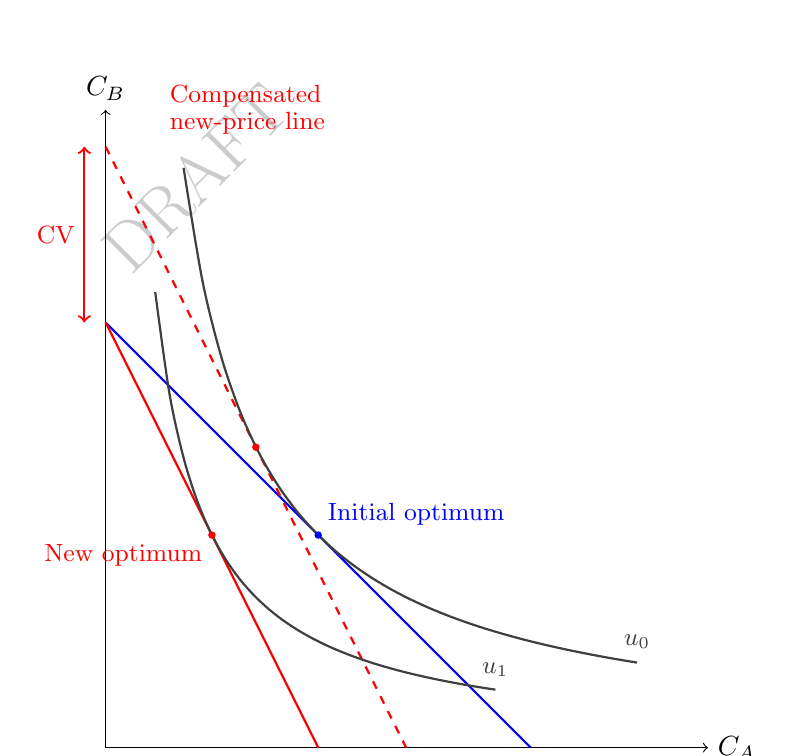
\begin{tikzpicture}[scale=0.9]
    % Axes
    \draw[->] (0,0) -- (8.5,0) node[right] {$C_A$};
    \draw[->] (0,0) -- (0,9.0) node[above] {$C_B$};

    % Budget lines
    \draw[thick, blue] (0,6) -- (6,0);


    \draw[thick, red] (0,6) -- (3,0);


    \draw[dashed, thick, red] (0,8.48) -- (4.24,0);
    \node[red, align=left] at (2.0,9.0) {\small Compensated\\[-0.5ex] \small new-price line};

    % Indifference curves
    \draw[domain=1.1:7.5,smooth,variable=\x, thick, darkgray] plot ({\x},{9/(\x)});
    \node[darkgray] at (7.5,1.5) {\small $u_0$};

    \draw[domain=0.7:5.5,smooth,variable=\x, thick, darkgray] plot ({\x},{4.5/(\x)});
    \node[darkgray] at (5.5,1.1) {\small $u_1$};

    % Tangency points
    \fill[blue] (3,3) circle (1.5pt) node[above right] {\small Initial optimum};
    \fill[red] (1.5,3) circle (1.5pt) node[below left] {\small New optimum};
    \fill[red] (2.12,4.24) circle (1.5pt);

    % CV arrow on vertical intercept
    \draw[<->, thick, red] (-0.3,6) -- (-0.3,8.48);
    \node[left, red] at (-0.3,7.24) {\small CV};
\end{tikzpicture}
\end{center}

\newpage
\paragraph{(ii) Equivalent variation.}
EV is the amount of income that could be taken away \emph{at the old prices} so that the consumer is just as badly off as after the price increase. Hence:
\begin{itemize}[leftmargin=*]
    \item the original budget line is tangent to \(u_0\);
    \item the new budget line is tangent to \(u_1\);
    \item an equivalent budget line, parallel to the original budget line, is shifted inward until it is tangent to \(u_1\).
\end{itemize}
The monetary gap between the original budget line and this inward-shifted old-price line is the equivalent variation.

\begin{center}
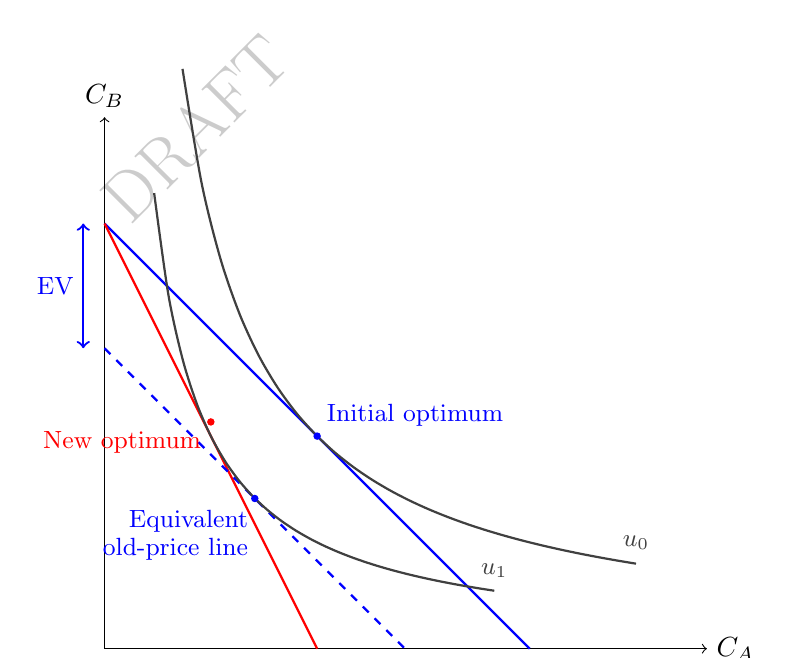
\begin{tikzpicture}[scale=0.9]
    % Axes
    \draw[->] (0,0) -- (8.5,0) node[right] {$C_A$};
    \draw[->] (0,0) -- (0,7.5) node[above] {$C_B$};

    % Budget lines
    \draw[thick, blue] (0,6) -- (6,0);


    \draw[thick, red] (0,6) -- (3,0);

    \draw[dashed, thick, blue] (0,4.24) -- (4.24,0);
    \node[blue, align=right] at (1,1.6) {\small Equivalent\\[-0.5ex] \small old-price line};

    % Indifference curves
    \draw[domain=1.1:7.5,smooth,variable=\x, thick, darkgray] plot ({\x},{9/(\x)});
    \node[darkgray] at (7.5,1.5) {\small $u_0$};

    \draw[domain=0.7:5.5,smooth,variable=\x, thick, darkgray] plot ({\x},{4.5/(\x)});
    \node[darkgray] at (5.5,1.1) {\small $u_1$};

    % Tangency points
    \fill[blue] (3,3) circle (1.5pt) node[above right] {\small Initial optimum};
    \fill[red] (1.5,3.2) circle (1.5pt) node[below left] {\small New optimum};
    \fill[blue] (2.12,2.12) circle (1.5pt);

    % EV arrow on vertical intercept
    \draw[<->, thick, blue] (-0.3,4.24) -- (-0.3,6);
    \node[left, blue] at (-0.3,5.12) {\small EV};
\end{tikzpicture}
\end{center}

These diagrams show the standard Hicksian welfare interpretation:
\[
\text{CV} = e(p_A',p_B,u_0)-e(p_A,p_B,u_0),
\qquad
\text{EV} = e(p_A,p_B,u_0)-e(p_A,p_B,u_1).
\]

\newpage
    \item
    For Cobb Douglas utility
    \[
    U(C_A,C_B)=C_A^{0.5}C_B^{0.5},
    \]
    the expenditure function is
    \[
    e(p_A,p_B,u)=2u\sqrt{p_Ap_B}.
    \]
    At the initial prices \((10,10)\) and income \(M=100\), the consumer spends half the income on each good, so
    \[
    C_A^*=\frac{50}{10}=5,
    \qquad
    C_B^*=\frac{50}{10}=5.
    \]
    Hence the initial utility is
    \[
    u_0=\sqrt{5\cdot 5}=5.
    \]

    CV is the extra income needed at the new prices \((20,10)\) to attain the original utility \(u_0=5\). Thus
    \[
    CV=e(20,10,5)-100.
    \]
    Compute:
    \[
    e(20,10,5)=2\cdot 5\sqrt{20\cdot 10}
    =10\sqrt{200}
    =10\cdot 10\sqrt{2}
    =100\sqrt{2}.
    \]
    Therefore
    \[
    CV=100\sqrt{2}-100=100(\sqrt{2}-1).
    \]
    Hence
    \[
    \boxed{CV=100(\sqrt{2}-1).}
    \]

    \item
    No, EV will not be equal to CV in this case.

    The reason is that Cobb Douglas preferences are \emph{not} quasilinear, so demand exhibits income effects. Fruit A is a normal good under Cobb Douglas preferences, and the price increase is harmful. For a price increase of a normal good, restoring the consumer to the original utility at the new prices is more expensive than measuring the equivalent utility loss at the old prices. Hence
    \[
    CV>EV.
    \]

    Therefore
    \[
    \boxed{EV\neq CV,\qquad CV>EV.}
    \]
\end{enumerate}

\newpage
\subsubsection{Method 2: Hicksian minimisation method}
\begin{enumerate}[label=(\alph*)]
    \item
    The graphical interpretation is the same as in Method 1.

    For CV, use the \emph{new} price slope and restore the \emph{old} indifference curve.  
    For EV, use the \emph{old} price slope and reduce income until the \emph{new} indifference curve is just reached.

    More precisely:
    \[
    \text{CV uses }(p_A',p_B)\text{ and }u_0,
    \qquad
    \text{EV uses }(p_A,p_B)\text{ and }u_1.
    \]

    \item
    At the initial prices \((10,10)\) and income \(100\), Cobb Douglas expenditure shares imply
    \[
    C_A^*=5,\qquad C_B^*=5,
    \]
    so
    \[
    u_0=\sqrt{5\cdot 5}=5.
    \]

    To compute CV, solve the Hicksian problem at the new prices:
    \[
    \min_{C_A,C_B>0}\;20C_A+10C_B
    \qquad\text{subject to}\qquad
    C_A^{0.5}C_B^{0.5}=5.
    \]
    Equivalently,
    \[
    C_AC_B=25.
    \]
    Substitute
    \[
    C_B=\frac{25}{C_A}
    \]
    into expenditure:
    \[
    E(C_A)=20C_A+10\left(\frac{25}{C_A}\right)
    =20C_A+\frac{250}{C_A}.
    \]
    Differentiate:
    \[
    E'(C_A)=20-\frac{250}{C_A^2}.
    \]
    Setting \(E'(C_A)=0\),
    \[
    20=\frac{250}{C_A^2}
    \quad\Longrightarrow\quad
    C_A^2=\frac{25}{2}
    \quad\Longrightarrow\quad
    C_A=\frac{5}{\sqrt2}.
    \]
    Then
    \[
    C_B=\frac{25}{5/\sqrt2}=5\sqrt2.
    \]
    Thus minimum expenditure is
    \[
    20\left(\frac{5}{\sqrt2}\right)+10(5\sqrt2)
    =50\sqrt2+50\sqrt2
    =100\sqrt2.
    \]
    Hence
    \[
    CV=100\sqrt2-100=100(\sqrt2-1).
    \]
    Therefore
    \[
    \boxed{CV=100(\sqrt2-1).}
    \]

    \item
    At the new prices \((20,10)\) and income \(100\), the Marshallian bundle is
    \[
    C_A'=\frac{50}{20}=2.5,
    \qquad
    C_B'=\frac{50}{10}=5.
    \]
    Hence the new utility is
    \[
    u_1=\sqrt{2.5\cdot 5}=\frac{5}{\sqrt2}.
    \]

    Since preferences are Cobb Douglas, there are income effects. Therefore EV and CV are not equal in general. Moreover, because fruit A is a normal good and its price rises,
    \[
    CV>EV.
    \]
    Hence
    \[
    \boxed{EV\neq CV,\qquad CV>EV.}
    \]
\end{enumerate}


%====================================================
% QUESTION 6 / Sample Question 2
%====================================================
\newpage
\section{Sample Question 2: Bob, Quasi-linear Utility, and Reservation Prices}

\noindent
Bob, who has wealth of \(w\) is deciding where to go for tea-time. There are \(3\) possible options, i) \(X\), ii) \(Y\), iii) \(Z\), and he can choose only \(1\) of the options.

\medskip

\noindent
If he chooses an option, its value is \(1\). If he does not choose the option, its value is \(0\). For example, if he chooses \(Y\), then \(X=0\), \(Y=1\), \(Z=0\) and so on.

\medskip

\noindent
His utility depends on which item he chooses and his leftover holdings of cash \(m\) as follows:
\[
u(X,Y,Z,m)=a\sqrt{X}+b\sqrt{Y}+c\sqrt{Z}+dm,
\]
where \(a,b,c,d>0\).

\subsection{Problem}
\begin{enumerate}[label=(\alph*)]
    \item State the definition of quasi-linear utility. Is Bob’s utility quasi-linear?
    \item Solve for Bob’s reservation prices for option \(X\), option \(Y\) and option \(Z\).
\end{enumerate}

\bigskip
\subsection{Solution}

\subsubsection{Method 1: Definition and indifference-pricing method}
\begin{enumerate}[label=(\alph*)]
    \item
    A utility function is \emph{quasi-linear} if it can be written in the form
    \[
    u(q,m)=\phi(q)+m
    \]
    up to a positive affine rescaling of the money variable, where utility is linear in one good, usually money.

    Here,
    \[
    u(X,Y,Z,m)=a\sqrt{X}+b\sqrt{Y}+c\sqrt{Z}+dm.
    \]
    Since \(d>0\), this is linear in money \(m\). Therefore Bob’s utility is quasi-linear. Equivalently, one may write
    \[
    u(X,Y,Z,m)=\phi(X,Y,Z)+dm,
    \]
    where
    \[
    \phi(X,Y,Z)=a\sqrt{X}+b\sqrt{Y}+c\sqrt{Z}.
    \]
    Hence
    \[
    \boxed{\text{Bob’s utility is quasi-linear.}}
    \]

\newpage
    \item
    Since \(X,Y,Z\in\{0,1\}\), we have
    \[
    \sqrt{X}=X,\qquad \sqrt{Y}=Y,\qquad \sqrt{Z}=Z.
    \]
    So the utility may be simplified to
    \[
    u(X,Y,Z,m)=aX+bY+cZ+dm.
    \]

    The reservation price for option \(X\) is the maximum amount Bob is willing to pay to choose \(X\) rather than choose no option. If he chooses no option, his utility is
    \[
    u(0,0,0,w)=dw.
    \]
    If he chooses option \(X\) and pays price \(r_X\), then his leftover cash is \(w-r_X\), so his utility is
    \[
    u(1,0,0,w-r_X)=a+d(w-r_X).
    \]
    At the reservation price he is indifferent:
    \[
    a+d(w-r_X)=dw.
    \]
    Hence
    \[
    dr_X=a
    \quad\Longrightarrow\quad
    \boxed{r_X=\frac{a}{d}.}
    \]

    Similarly, for option \(Y\),
    \[
    u(0,1,0,w-r_Y)=b+d(w-r_Y),
    \]
    and indifference with choosing no option gives
    \[
    b+d(w-r_Y)=dw
    \quad\Longrightarrow\quad
    \boxed{r_Y=\frac{b}{d}.}
    \]

    Likewise, for option \(Z\),
    \[
    u(0,0,1,w-r_Z)=c+d(w-r_Z),
    \]
    so
    \[
    c+d(w-r_Z)=dw
    \quad\Longrightarrow\quad
    \boxed{r_Z=\frac{c}{d}.}
    \]

    Therefore
    \[
    \boxed{
    r_X=\frac{a}{d},\qquad
    r_Y=\frac{b}{d},\qquad
    r_Z=\frac{c}{d}.
    }
    \]
\end{enumerate}

\newpage
\subsubsection{Method 2: Utility-value conversion method}
\begin{enumerate}[label=(\alph*)]
    \item
    A utility function is quasi-linear if utility is linear in one argument, typically money. Here
    \[
    u(X,Y,Z,m)=a\sqrt{X}+b\sqrt{Y}+c\sqrt{Z}+dm
    \]
    is linear in \(m\), so Bob’s utility is quasi-linear.

    Hence
    \[
    \boxed{\text{Bob’s utility is quasi-linear.}}
    \]

    \item
    Since one extra dollar of leftover cash raises utility by
    \[
    d,
    \]
    the marginal utility of money is \(d\). Therefore a utility increment of size \(\Delta u\) has money equivalent
    \[
    \frac{\Delta u}{d}.
    \]

    Now the utility bonus from choosing option \(X\) rather than no option is
    \[
    a\sqrt{1}=a.
    \]
    So its reservation price is
    \[
    \boxed{r_X=\frac{a}{d}.}
    \]

    Similarly, option \(Y\) gives utility bonus
    \[
    b\sqrt{1}=b,
    \]
    so
    \[
    \boxed{r_Y=\frac{b}{d}.}
    \]

    Option \(Z\) gives utility bonus
    \[
    c\sqrt{1}=c,
    \]
    so
    \[
    \boxed{r_Z=\frac{c}{d}.}
    \]

    Therefore
    \[
    \boxed{
    r_X=\frac{a}{d},\qquad
    r_Y=\frac{b}{d},\qquad
    r_Z=\frac{c}{d}.
    }
    \]
\end{enumerate}

\newpage
\subsubsection{Method 3: Binary-choice simplification method}
\begin{enumerate}[label=(\alph*)]
    \item
    Because each of \(X,Y,Z\) is binary,
    \[
    X,Y,Z\in\{0,1\},
    \]
    the square-root terms simplify exactly:
    \[
    \sqrt{X}=X,\qquad \sqrt{Y}=Y,\qquad \sqrt{Z}=Z.
    \]
    Hence Bob’s utility can be rewritten as
    \[
    u(X,Y,Z,m)=aX+bY+cZ+dm.
    \]
    This is of quasi-linear form: an additive term depending on the discrete choice variables plus a linear money term.

    Therefore
    \[
    \boxed{\text{Bob’s utility is quasi-linear.}}
    \]

    \item
    In the simplified form
    \[
    u(X,Y,Z,m)=aX+bY+cZ+dm,
    \]
    choosing no option yields utility
    \[
    dw.
    \]
    Choosing option \(X\) and paying price \(p\) yields
    \[
    a+d(w-p).
    \]
    Bob is indifferent when
    \[
    a+d(w-p)=dw
    \quad\Longrightarrow\quad
    p=\frac{a}{d}.
    \]
    So
    \[
    \boxed{r_X=\frac{a}{d}.}
    \]

    Repeating the same argument for \(Y\) and \(Z\),
    \[
    \boxed{r_Y=\frac{b}{d},\qquad r_Z=\frac{c}{d}.}
    \]

    Therefore
    \[
    \boxed{
    r_X=\frac{a}{d},\qquad
    r_Y=\frac{b}{d},\qquad
    r_Z=\frac{c}{d}.
    }
    \]
\end{enumerate}

\newpage
\part{Tutorial 8}
\section{Sample Question 1: Good X with Heterogeneous Consumers and Firms}

\subsection{Problem}

\noindent
In the market for good \(X\), which has a price of \(p\), there are 160 consumers with an identical income of \$100. There are two types of consumers, Type 1 and Type 2, each with different preferences.

\noindent
Type 1s have preferences
\[
U_1(x)=16x-4x^2+m,
\]
where \(x\) is the quantity of good \(x\) purchased and \(m\) is their leftover cash holdings. Type 2s have preferences
\[
U_2(x)=8x-8x^2+m.
\]

\bigskip
\noindent There are 80 consumers of Type 1 and 80 consumers of Type 2.

\begin{enumerate}[label=(\alph*)]
    \item Derive the individual demand curves for Type 1 and Type 2 consumers. \hfill \textbf{(6 marks)}
    \item Derive the aggregate demand curve for good \(X\). \hfill \textbf{(5 marks)}
\end{enumerate}


\bigskip
\noindent
In the market for good \(X\), there are also a total of \(n\) identical firms who are profit maximisers. Each of these firms has a cost function of$3x^2.$
\begin{enumerate}[label=(\alph*), start=3]
    \item Maximise the profits of each firm \((px-3x^2)\) to derive the individual supply curve. Subsequently derive the aggregate supply curve for good \(X\). \hfill \textbf{(5 marks)}
    \item How does the market’s elasticity of supply change with the number of firms in the market? Explain. \hfill \textbf{(4 marks)}
\end{enumerate}

\bigskip
\noindent
Suppose that \(n=72\), i.e. there are 72 firms in the market.

\begin{enumerate}[label=(\alph*), start=5]
    \item Draw out the aggregate demand and supply curves in the market, calculating and indicating the exact market equilibrium on your figure. \hfill \textbf{(7 marks)}
    \item What is the amount of consumer and producer surplus in the market? \hfill \textbf{(5 marks)}
\end{enumerate}

\noindent
Suppose that the government now imposes a per unit tax of \$6 on producers.

\begin{enumerate}[label=(\alph*), start=7]
    \item Illustrate in a diagram, as accurately as possible, the effect of the tax, indicating i) the deadweight welfare loss, and ii) the incidence of the tax burden on consumers and producers. \hfill \textbf{(8 marks)}
\end{enumerate}


\newpage
\subsection{Solution}

\subsubsection{Method 1: Direct optimisation, aggregation, and equilibrium solving}

\begin{enumerate}[label=(\alph*)]
    \item
    For Type 1, since leftover cash is
    \[
    m=100-px,
    \]
    utility becomes
    \[
    U_1(x)=16x-4x^2+100-px.
    \]
    Differentiate:
    \[
    \frac{dU_1}{dx}=16-8x-p.
    \]
    Setting the first-order condition equal to zero,
    \[
    16-8x-p=0
    \quad\Longrightarrow\quad
    x=\frac{16-p}{8}=2-\frac{p}{8}.
    \]
    Because
    \[
    \frac{d^2U_1}{dx^2}=-8<0,
    \]
    this is the maximiser whenever it is nonnegative. Hence
    \[
    x_1(p)=
    \begin{cases}
    2-\dfrac{p}{8}, & 0\le p\le 16,\\[0.6em]
    0, & p>16.
    \end{cases}
    \]

    For Type 2,
    \[
    U_2(x)=8x-8x^2+100-px.
    \]
    Differentiate:
    \[
    \frac{dU_2}{dx}=8-16x-p.
    \]
    Setting this equal to zero,
    \[
    8-16x-p=0
    \quad\Longrightarrow\quad
    x=\frac{8-p}{16}=\frac12-\frac{p}{16}.
    \]
    Since
    \[
    \frac{d^2U_2}{dx^2}=-16<0,
    \]
    this is the maximiser whenever nonnegative. Therefore
    \[
    x_2(p)=
    \begin{cases}
    \dfrac12-\dfrac{p}{16}, & 0\le p\le 8,\\[0.6em]
    0, & p>8.
    \end{cases}
    \]

    Thus
    \[
    \boxed{
    x_1(p)=
    \begin{cases}
    2-\dfrac{p}{8}, & 0\le p\le 16,\\[0.5em]
    0, & p>16,
    \end{cases}
    \qquad
    x_2(p)=
    \begin{cases}
    \dfrac12-\dfrac{p}{16}, & 0\le p\le 8,\\[0.5em]
    0, & p>8.
    \end{cases}}
    \]

    \item
    There are 80 consumers of each type, so aggregate demand is
    \[
    Q_D(p)=80x_1(p)+80x_2(p).
    \]

    For \(0\le p\le 8\), both types buy:
    \begin{align*}
    Q_D(p)
    &=80\left(2-\frac{p}{8}\right)+80\left(\frac12-\frac{p}{16}\right)\\
    &=160-10p+40-5p\\
    &=200-15p.
    \end{align*}

    For \(8<p\le 16\), only Type 1 buys:
    \[
    Q_D(p)=80\left(2-\frac{p}{8}\right)=160-10p.
    \]

    For \(p>16\), nobody buys:
    \[
    Q_D(p)=0.
    \]

    Hence
    \[
    \boxed{
    Q_D(p)=
    \begin{cases}
    200-15p, & 0\le p\le 8,\\[0.4em]
    160-10p, & 8<p\le 16,\\[0.4em]
    0, & p>16.
    \end{cases}}
    \]

    \item
    Each firm solves
    \[
    \max_{x\ge 0}\; \pi(x)=px-3x^2.
    \]
    Differentiate:
    \[
    \frac{d\pi}{dx}=p-6x.
    \]
    Setting this equal to zero,
    \[
    p-6x=0
    \quad\Longrightarrow\quad
    x=\frac{p}{6}.
    \]
    Since
    \[
    \frac{d^2\pi}{dx^2}=-6<0,
    \]
    this is the profit-maximising quantity. Therefore the individual supply curve is
    \[
    \boxed{x_s(p)=\frac{p}{6}.}
    \]

    With \(n\) identical firms, aggregate supply is
    \[
    Q_S(p)=n\frac{p}{6}.
    \]
    So
    \[
    \boxed{Q_S(p)=\frac{n}{6}p.}
    \]

    \item
    Since
    \[
    Q_S(p)=\frac{n}{6}p,
    \]
    we have
    \[
    \frac{dQ_S}{dp}=\frac{n}{6}.
    \]
    The price elasticity of supply is
    \[
    \varepsilon_S=\frac{dQ_S}{dp}\cdot \frac{p}{Q_S(p)}
    =\frac{n}{6}\cdot \frac{p}{(n/6)p}=1.
    \]
    Hence the market’s elasticity of supply does not change with the number of firms:
    \[
    \boxed{\varepsilon_S=1\text{ for all }p>0.}
    \]

    The number of firms changes the scale of market supply, but not its elasticity.

    \item
    Set \(n=72\). Then market supply is
    \[
    Q_S(p)=\frac{72}{6}p=12p.
    \]
    Since the equilibrium price will turn out to be below 8, the relevant demand branch is
    \[
    Q_D(p)=200-15p.
    \]
    Equating demand and supply,
    \[
    200-15p=12p.
    \]
    Hence
    \[
    27p=200
    \quad\Longrightarrow\quad
    p^*=\frac{200}{27}.
    \]
    Therefore
    \[
    Q^*=12p^*=\frac{800}{9}.
    \]

    Thus
    \[
    \boxed{p^*=\frac{200}{27},\qquad Q^*=\frac{800}{9}.}
    \]

    A suitable graph is:

    \begin{center}
    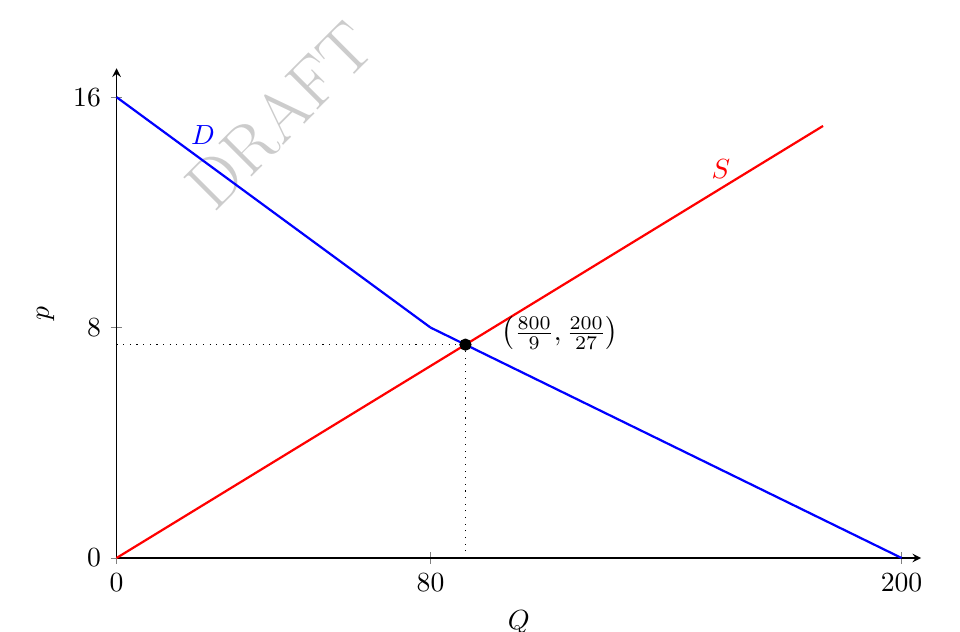
\begin{tikzpicture}
    \begin{axis}[
        width=11.8cm,
        height=7.8cm,
        xmin=0,xmax=205,
        ymin=0,ymax=17,
        axis lines=left,
        xlabel={$Q$},
        ylabel={$p$},
        xtick={0,80,200},
        xticklabels={$0$,$80$,$200$},
        ytick={0,8,16},
        yticklabels={$0$,$8$,$16$},
        clip=false
    ]
    \addplot[thick,blue] coordinates {(0,16) (80,8)};
    \addplot[thick,blue] coordinates {(80,8) (200,0)};
    \addplot[thick,red,domain=0:180,samples=2] {x/12};

    \addplot[dotted] coordinates {(88.8889,0) (88.8889,7.4074)};
    \addplot[dotted] coordinates {(0,7.4074) (88.8889,7.4074)};
    \addplot[only marks,mark=*,mark size=2pt] coordinates {(88.8889,7.4074)};

    \node[blue] at (axis cs:22,14.7) {$D$};
    \node[red] at (axis cs:154,13.5) {$S$};
    \node at (axis cs:113,7.8) {$\left(\frac{800}{9},\frac{200}{27}\right)$};
    \end{axis}
    \end{tikzpicture}
    \end{center}

    \item
    At the equilibrium price \(p^*=\frac{200}{27}\), Type 1 buys
    \[
    x_1^*=2-\frac{1}{8}\cdot \frac{200}{27}
    =2-\frac{25}{27}
    =\frac{29}{27},
    \]
    while Type 2 buys
    \[
    x_2^*=\frac12-\frac{1}{16}\cdot \frac{200}{27}
    =\frac12-\frac{25}{54}
    =\frac{1}{27}.
    \]

    Type 1 consumer surplus per consumer is
    \[
    CS_1^{\text{ind}}
    =\frac12\left(16-\frac{200}{27}\right)\frac{29}{27}
    =\frac{3364}{729}.
    \]
    Across 80 Type 1 consumers:
    \[
    CS_1=80\cdot \frac{3364}{729}=\frac{269120}{729}.
    \]

    Type 2 consumer surplus per consumer is
    \[
    CS_2^{\text{ind}}
    =\frac12\left(8-\frac{200}{27}\right)\frac{1}{27}
    =\frac{8}{729}.
    \]
    Across 80 Type 2 consumers:
    \[
    CS_2=80\cdot \frac{8}{729}=\frac{640}{729}.
    \]

    Therefore
    \[
    CS=CS_1+CS_2=\frac{269760}{729}=\frac{89920}{243}.
    \]
    So
    \[
    \boxed{CS=\frac{89920}{243}.}
    \]

    Producer surplus is
    \[
    PS=\frac12 p^*Q^*
    =\frac12\cdot \frac{200}{27}\cdot \frac{800}{9}
    =\frac{80000}{243}.
    \]
    Hence
    \[
    \boxed{PS=\frac{80000}{243}.}
    \]

    \item
    A per-unit tax of \(6\) on producers implies
    \[
    p_b=p_s+6.
    \]
    Since aggregate supply before tax is
    \[
    Q_S=12p_s,
    \]
    aggregate supply in terms of the buyers' price is
    \[
    Q_S^t(p_b)=12(p_b-6)=12p_b-72.
    \]
    After tax the buyers' price exceeds 8, so only Type 1 remains active. Hence the relevant demand branch is
    \[
    Q_D(p_b)=160-10p_b.
    \]
    Equating demand and taxed supply,
    \[
    160-10p_b=12p_b-72.
    \]
    Therefore
    \[
    232=22p_b
    \quad\Longrightarrow\quad
    p_b=\frac{116}{11}.
    \]
    The taxed quantity is
    \[
    Q_t=160-10p_b=\frac{600}{11},
    \]
    and the sellers' net price is
    \[
    p_s=p_b-6=\frac{50}{11}.
    \]

    Thus
    \[
    \boxed{p_b=\frac{116}{11},\qquad p_s=\frac{50}{11},\qquad Q_t=\frac{600}{11}.}
    \]

    The consumer burden is
    \[
    p_b-p^*=\frac{116}{11}-\frac{200}{27}=\frac{932}{297},
    \]
    while the producer burden is
    \[
    p^*-p_s=\frac{200}{27}-\frac{50}{11}=\frac{850}{297}.
    \]
    The deadweight loss is
    \[
    DWL=\frac12\cdot 6\left(\frac{800}{9}-\frac{600}{11}\right)
    =\frac{3400}{33}.
    \]
    Hence
    \[
    \boxed{\text{consumer burden}=\frac{932}{297},\quad \text{producer burden}=\frac{850}{297},\quad DWL=\frac{3400}{33}.}
    \]

    A suitable tax diagram is:

    \begin{center}
    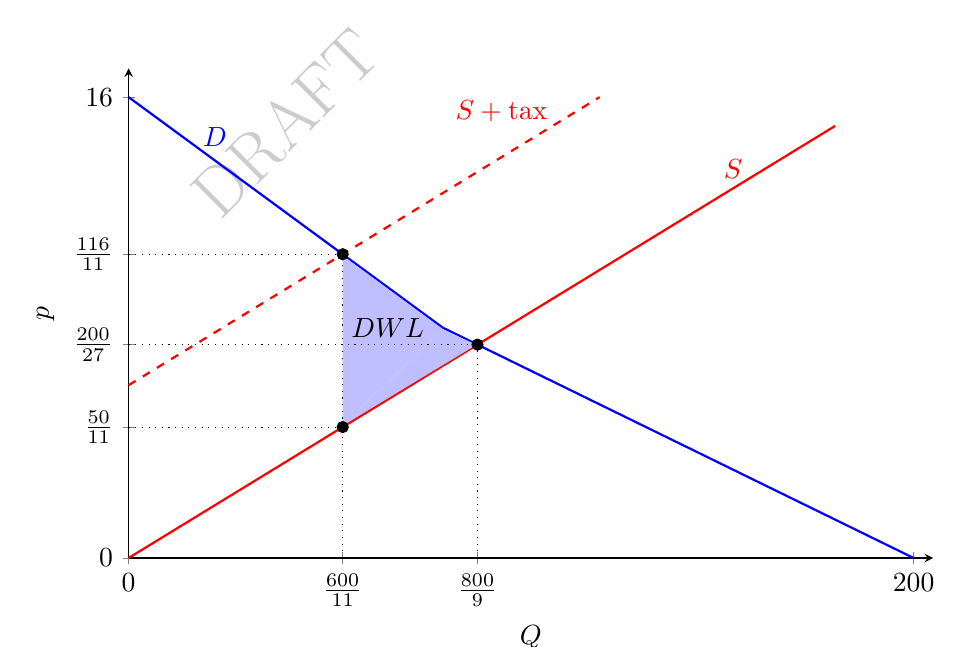
\begin{tikzpicture}
    \begin{axis}[
        width=11.8cm,
        height=7.8cm,
        xmin=0,xmax=205,
        ymin=0,ymax=17,
        axis lines=left,
        xlabel={$Q$},
        ylabel={$p$},
        xtick={0,54.5455,88.8889,200},
        xticklabels={$0$,$\frac{600}{11}$,$\frac{800}{9}$,$200$},
        ytick={0,4.5455,7.4074,10.5455,16},
        yticklabels={$0$,$\frac{50}{11}$,$\frac{200}{27}$,$\frac{116}{11}$,$16$},
        clip=false
    ]
    \addplot[thick,blue] coordinates {(0,16) (80,8)};
    \addplot[thick,blue] coordinates {(80,8) (200,0)};
    \addplot[thick,red,domain=0:180,samples=2] {x/12};
    \addplot[thick,red,dashed,domain=0:120,samples=2] {6 + x/12};

    \addplot[fill=blue!25,draw=none]
        coordinates {(54.5455,4.6) (54.5455,10.5) (80,7.95) (54.5455,4.6)};
    
    \addplot[fill=blue!25,draw=none]
        coordinates {(54.5455,4.6) (80,7.95) (88.6,7.4) (54.5455,4.6)};

    \addplot[dotted] coordinates {(88.8889,0) (88.8889,7.4074)};
    \addplot[dotted] coordinates {(54.5455,0) (54.5455,10.5455)};
    \addplot[dotted] coordinates {(0,10.5455) (54.5455,10.5455)};
    \addplot[dotted] coordinates {(0,4.5455) (54.5455,4.5455)};
    \addplot[dotted] coordinates {(0,7.4074) (88.8889,7.4074)};

    \addplot[only marks,mark=*,mark size=2pt]
        coordinates {(88.8889,7.4074) (54.5455,10.5455) (54.5455,4.5455)};

    \node[blue] at (axis cs:22,14.6) {$D$};
    \node[red] at (axis cs:154,13.5) {$S$};
    \node[red] at (axis cs:95,15.5) {$S+\text{tax}$};
    \node at (axis cs:66,8.0) {$DWL$};
    \end{axis}
    \end{tikzpicture}
    \end{center}
\end{enumerate}

\newpage
\subsubsection{Method 2: Inverse-demand / inverse-supply and welfare geometry}

\begin{enumerate}[label=(\alph*)]
    \item
    The individual demand curves can be written compactly as
    \[
    x_1(p)=\left(2-\frac{p}{8}\right)_+,
    \qquad
    x_2(p)=\left(\frac12-\frac{p}{16}\right)_+,
    \]
    where \((z)_+=\max\{z,0\}\). Equivalently,
    \[
    \boxed{
    x_1(p)=
    \begin{cases}
    2-\dfrac{p}{8}, & 0\le p\le 16,\\
    0, & p>16,
    \end{cases}
    \qquad
    x_2(p)=
    \begin{cases}
    \dfrac12-\dfrac{p}{16}, & 0\le p\le 8,\\
    0, & p>8.
    \end{cases}}
    \]

    \item
    Aggregate demand is
    \[
    Q_D(p)=80\left(2-\frac{p}{8}\right)_+ + 80\left(\frac12-\frac{p}{16}\right)_+.
    \]
    Inverse demand is therefore piecewise:
    \[
    p_D(Q)=
    \begin{cases}
    16-\dfrac{Q}{10}, & 0\le Q\le 80,\\[0.7em]
    \dfrac{200-Q}{15}, & 80\le Q\le 200.
    \end{cases}
    \]
    Hence
    \[
    \boxed{
    p_D(Q)=
    \begin{cases}
    16-\dfrac{Q}{10}, & 0\le Q\le 80,\\[0.7em]
    \dfrac{200-Q}{15}, & 80\le Q\le 200.
    \end{cases}}
    \]

    \item
    Each firm has cost \(3x^2\), so marginal cost is
    \[
    MC(x)=6x.
    \]
    Competitive supply satisfies \(p=MC\), so
    \[
    x_s(p)=\frac{p}{6}.
    \]
    Aggregating across \(n\) firms gives
    \[
    Q_S(p)=\frac{n}{6}p,
    \qquad
    p_S(Q)=\frac{6Q}{n}.
    \]
    Therefore
    \[
    \boxed{Q_S(p)=\frac{n}{6}p,\qquad p_S(Q)=\frac{6Q}{n}.}
    \]

    \item
    Because \(Q_S(p)\) is proportional to \(p\), its elasticity is identically 1:
    \[
    \varepsilon_S=\frac{dQ_S}{dp}\cdot \frac{p}{Q_S}=1.
    \]
    Hence
    \[
    \boxed{\varepsilon_S=1.}
    \]

    \item
    For \(n=72\),
    \[
    p_S(Q)=\frac{Q}{12}.
    \]
    Solve using the lower branch of inverse demand:
    \[
    \frac{200-Q}{15}=\frac{Q}{12}.
    \]
    Therefore
    \[
    12(200-Q)=15Q
    \quad\Longrightarrow\quad
    2400=27Q
    \quad\Longrightarrow\quad
    Q^*=\frac{800}{9}.
    \]
    Then
    \[
    p^*=\frac{Q^*}{12}=\frac{200}{27}.
    \]
    Thus
    \[
    \boxed{Q^*=\frac{800}{9},\qquad p^*=\frac{200}{27}.}
    \]

    \item
    Consumer surplus is the area under inverse demand above price:
    \begin{align*}
    CS
    &=\int_0^{80}\left(16-\frac{Q}{10}\right)\,dQ
      +\int_{80}^{800/9}\left(\frac{200-Q}{15}\right)\,dQ
      -\frac{200}{27}\cdot \frac{800}{9}\\
    &=\frac{89920}{243}.
    \end{align*}
    Producer surplus is
    \[
    PS=\frac12 Q^*p^*
    =\frac12\cdot \frac{800}{9}\cdot \frac{200}{27}
    =\frac{80000}{243}.
    \]
    Hence
    \[
    \boxed{CS=\frac{89920}{243},\qquad PS=\frac{80000}{243}.}
    \]

    \item
    A tax of 6 on producers shifts inverse supply vertically upward by 6:
    \[
    p_{S,t}(Q)=\frac{Q}{12}+6.
    \]
    After tax, the relevant demand branch is the upper one:
    \[
    16-\frac{Q}{10}=\frac{Q}{12}+6.
    \]
    Solving,
    \[
    10=\frac{11Q}{60}
    \quad\Longrightarrow\quad
    Q_t=\frac{600}{11}.
    \]
    Therefore
    \[
    p_b=16-\frac{Q_t}{10}=\frac{116}{11},
    \qquad
    p_s=p_b-6=\frac{50}{11}.
    \]
    The deadweight loss is
    \[
    DWL=\frac12\cdot 6\left(\frac{800}{9}-\frac{600}{11}\right)=\frac{3400}{33}.
    \]
    Thus
    \[
    \boxed{Q_t=\frac{600}{11},\qquad p_b=\frac{116}{11},\qquad p_s=\frac{50}{11},\qquad DWL=\frac{3400}{33}.}
    \]
\end{enumerate}

\newpage
\subsubsection{Method 3: Comparative-statics / elasticity and regime-switch method}

\begin{enumerate}[label=(\alph*)]
    \item
    Write individual demands as
    \[
    x_1(p)=\left(2-\frac{p}{8}\right)_+,
    \qquad
    x_2(p)=\left(\frac12-\frac{p}{16}\right)_+.
    \]
    The cutoffs are therefore
    \[
    p=16 \quad\text{for Type 1,}
    \qquad
    p=8 \quad\text{for Type 2.}
    \]
    So Type 2 exits first as price rises.

    \item
    Aggregate demand is
    \[
    Q_D(p)=80\left(2-\frac{p}{8}\right)_+ + 80\left(\frac12-\frac{p}{16}\right)_+,
    \]
    which gives the two active regimes
    \[
    Q_D(p)=200-15p \quad (0\le p\le 8),
    \qquad
    Q_D(p)=160-10p \quad (8<p\le 16).
    \]
    The structural point is that the demand slope changes when Type 2 exits.

    \item
    Supply is
    \[
    Q_S(p)=\frac{n}{6}p,
    \]
    so changing \(n\) rotates market supply outward through the origin.

    \item
    Even though changing \(n\) changes the level of market supply, the elasticity remains
    \[
    \varepsilon_S=1.
    \]
    Thus
    \[
    \boxed{\text{more firms } \Rightarrow \text{ more supply at each price, but the same elasticity}.}
    \]

    \item
    To determine which demand branch is relevant, compare the supply quantity at \(p=8\):
    \[
    Q_S(8)=\frac{n}{6}\cdot 8=\frac{4n}{3}.
    \]
    If both types are active, then the branch switch occurs at the market kink \((Q,p)=(80,8)\). Hence:
    \[
    \frac{4n}{3} \gtrless 80
    \quad\Longleftrightarrow\quad
    n \gtrless 60.
    \]
    So:
    \begin{itemize}[leftmargin=*]
        \item if \(n>60\), equilibrium lies on the lower branch \(Q_D=200-15p\);
        \item if \(n<60\), equilibrium lies on the upper branch \(Q_D=160-10p\);
        \item if \(n=60\), equilibrium is exactly at the kink.
    \end{itemize}
    Since \(n=72>60\), we use
    \[
    200-15p=12p,
    \]
    which yields
    \[
    \boxed{p^*=\frac{200}{27},\qquad Q^*=\frac{800}{9}.}
    \]

    \item
    Since \(Q^*=\frac{800}{9}>80\), both consumer types remain active in the no-tax equilibrium, but Type 2 buys only a very small amount:
    \[
    x_2^*=\frac{1}{27}.
    \]
    This already suggests that a sufficiently strong tax can push Type 2 completely out of the market.

    Using the area formulas on the aggregate curves,
    \[
    \boxed{CS=\frac{89920}{243},\qquad PS=\frac{80000}{243}.}
    \]

    \item
    After a producer tax \(t=6\), buyer-price supply becomes
    \[
    Q_S^t(p_b)=\frac{n}{6}(p_b-6).
    \]
    For \(n=72\),
    \[
    Q_S^t(p_b)=12p_b-72.
    \]
    Check what happens at the demand cutoff \(p_b=8\):
    \[
    Q_S^t(8)=24,
    \qquad
    Q_D(8)=80.
    \]
    Since taxed supply at \(p_b=8\) is far below demand at the kink, the post-tax equilibrium must occur on the upper branch where only Type 1 remains active. Hence solve
    \[
    160-10p_b=12p_b-72.
    \]
    Therefore
    \[
    \boxed{p_b=\frac{116}{11},\qquad p_s=\frac{50}{11},\qquad Q_t=\frac{600}{11}.}
    \]

    The key comparative-statics insight is that the tax does more than just reduce quantity: it changes the active set of consumers. Type 2 exits completely after tax. The resulting deadweight loss is
    \[
    \boxed{DWL=\frac{3400}{33}.}
    \]
\end{enumerate}

\newpage
\subsubsection{Marking scheme (40 marks)}

\begin{enumerate}[label=(\alph*)]
    \item \textbf{(6 marks)} Individual demand curves
    \begin{itemize}
        \item 2 marks: Correct setup of the Type 1 utility-maximisation problem, including substitution of leftover cash \(m=100-px\) or an equivalent formulation.
        \item 2 marks: Correct derivation of the Type 1 demand curve, including the non-negativity condition.
        \item 2 marks: Correct derivation of the Type 2 demand curve, including the non-negativity condition.
    \end{itemize}

    \item \textbf{(5 marks)} Aggregate demand curve
    \begin{itemize}
        \item 2 marks: Correct identification of the relevant price regions and which consumer types are active in each region.
        \item 2 marks: Correct piecewise aggregation of the two individual demand curves.
        \item 1 mark: Correct final aggregate demand curve, including the kink / cutoff structure.
    \end{itemize}

    \item \textbf{(5 marks)} Individual and aggregate supply
    \begin{itemize}
        \item 2 marks: Correct setup of the firm’s profit-maximisation problem.
        \item 1 mark: Correct individual supply curve.
        \item 2 marks: Correct aggregate supply curve for \(n\) identical firms.
    \end{itemize}

    \item \textbf{(4 marks)} Market elasticity of supply
    \begin{itemize}
        \item 2 marks: Correct elasticity result, including whether it changes with the number of firms.
        \item 2 marks: Clear economic explanation of why the elasticity does or does not change as \(n\) varies.
    \end{itemize}

    \item \textbf{(7 marks)} Equilibrium for \(n=72\)
    \begin{itemize}
        \item 2 marks: Correct substitution of \(n=72\) into the aggregate supply curve.
        \item 2 marks: Correct identification of the relevant branch of aggregate demand.
        \item 2 marks: Correct equilibrium price and quantity.
        \item 1 mark: Diagram with demand, supply, and the exact equilibrium correctly indicated.
    \end{itemize}

    \item \textbf{(5 marks)} Consumer and producer surplus
    \begin{itemize}
        \item 2 marks: Correct computation of consumer surplus.
        \item 2 marks: Correct computation of producer surplus.
        \item 1 mark: Correct final expressions / values, consistent with the equilibrium from part (e).
    \end{itemize}

    \item \textbf{(8 marks)} Per-unit tax on producers
    \begin{itemize}
        \item 2 marks: Correct setup of the post-tax equilibrium, including the tax wedge between buyers’ and sellers’ prices.
        \item 2 marks: Correct taxed prices and quantity, or a fully correct equivalent derivation.
        \item 2 marks: Correct deadweight welfare loss, or a correct DWL triangle with correct dimensions.
        \item 2 marks: Diagram and explanation correctly showing the incidence of the tax burden on consumers and producers.
    \end{itemize}
\end{enumerate}

%====================================================
% Sample Question 2
%====================================================
\newpage
\section{Sample Question 2: Teddy Bears}

\subsection{Problem}

\noindent
Consider the market for teddy bears. \footnote{There appears to be a likely typo in the handout. If the individual supply curve is written as \(S(p)=4p-100\), then positive supply requires \(p\ge 25\), while market demand \(D(p)=1000-80p\) falls to zero at \(p=12.5\). Hence there is no interior trade equilibrium, so the later tax and deadweight-loss parts become degenerate. The intended version is very likely \(S(p)=4p-10\), which yields a standard non-degenerate competitive-equilibrium and welfare-analysis problem.} There are \(n\) firms with \emph{individual} supply curves given by
\[
S(p)=4p-10.
\]
The \emph{market} demand curve is given by
\[
D(p)=1000-80p.
\]

\begin{enumerate}[label=(\alph*)]
    \item Derive the market supply curve in terms of \(n\). \hfill \textbf{(5 marks)}
    \item Suppose there is a per-unit tax of \$5 on the \emph{consumers}. For \(n=10\), draw out the market supply and demand curves \emph{with} and \emph{without} tax, indicating and explaining the deadweight welfare loss from the tax. \hfill \textbf{(9 marks)}
    \item For the same per-unit tax on consumers, calculate the deadweight welfare loss as a function of the number of producers in the market \(n\). \hfill \textbf{(10 marks)}
    \item How does the deadweight welfare loss change with the number of producers? Explain the intuition behind this. \hfill \textbf{(6 marks)}
\end{enumerate}

\newpage
\subsection{Solution}

\subsubsection{Method 1: Direct aggregation and tax-wedge algebra}

\begin{enumerate}[label=(\alph*)]
    \item
    Each firm supplies
    \[
    q_i(p)=4p-10.
    \]
    With \(n\) identical firms, market supply is
    \[
    Q_S(p)=n(4p-10)=4np-10n.
    \]
    Therefore
    \[
    \boxed{Q_S(p)=4np-10n.}
    \]

    \item
    For \(n=10\), the market supply curve is
    \[
    Q_S(p)=40p-100.
    \]
    Demand is
    \[
    Q_D(p)=1000-80p.
    \]

    Before tax, equilibrium satisfies
    \[
    1000-80p=40p-100.
    \]
    Hence
    \[
    1100=120p
    \quad\Longrightarrow\quad
    p^*=\frac{55}{6}.
    \]
    Then
    \[
    Q^*=1000-80p^*
    =1000-80\cdot \frac{55}{6}
    =\frac{800}{3}.
    \]

    Thus
    \[
    \boxed{p^*=\frac{55}{6},\qquad Q^*=\frac{800}{3}.}
    \]

    Now impose a per-unit tax of 5 on consumers. Let \(p_b\) be the buyers' price and \(p_s\) the sellers' price. Then
    \[
    p_b=p_s+5.
    \]
    Demand is
    \[
    Q_D=1000-80p_b,
    \]
    while supply depends on the sellers' price:
    \[
    Q_S=40p_s-100.
    \]
    Substitute \(p_s=p_b-5\):
    \[
    Q_S=40(p_b-5)-100=40p_b-300.
    \]
    Equate demand and supply:
    \[
    1000-80p_b=40p_b-300.
    \]
    Hence
    \[
    1300=120p_b
    \quad\Longrightarrow\quad
    p_b=\frac{65}{6}.
    \]
    Therefore
    \[
    p_s=p_b-5=\frac{35}{6}.
    \]
    The taxed quantity is
    \[
    Q_t=1000-80p_b
    =1000-80\cdot \frac{65}{6}
    =\frac{400}{3}.
    \]

    Thus
    \[
    \boxed{p_b=\frac{65}{6},\qquad p_s=\frac{35}{6},\qquad Q_t=\frac{400}{3}.}
    \]

    The deadweight loss is
    \(
    DWL=\frac12\cdot 5\left(\frac{800}{3}-\frac{400}{3}\right)=\frac{1000}{3}.
    \)
    Hence $\quad \boxed{DWL=\frac{1000}{3}.}$

    A suitable graph\footnote{Although the solution represents the consumer tax as an upward shift of supply, an equivalent and often clearer representation is a downward shift of demand, which more directly reflects the tax being levied on consumers. Both approaches impose the same wedge \(p_b - p_s = t\) and yield identical equilibrium outcomes.} is:

    \begin{center}
    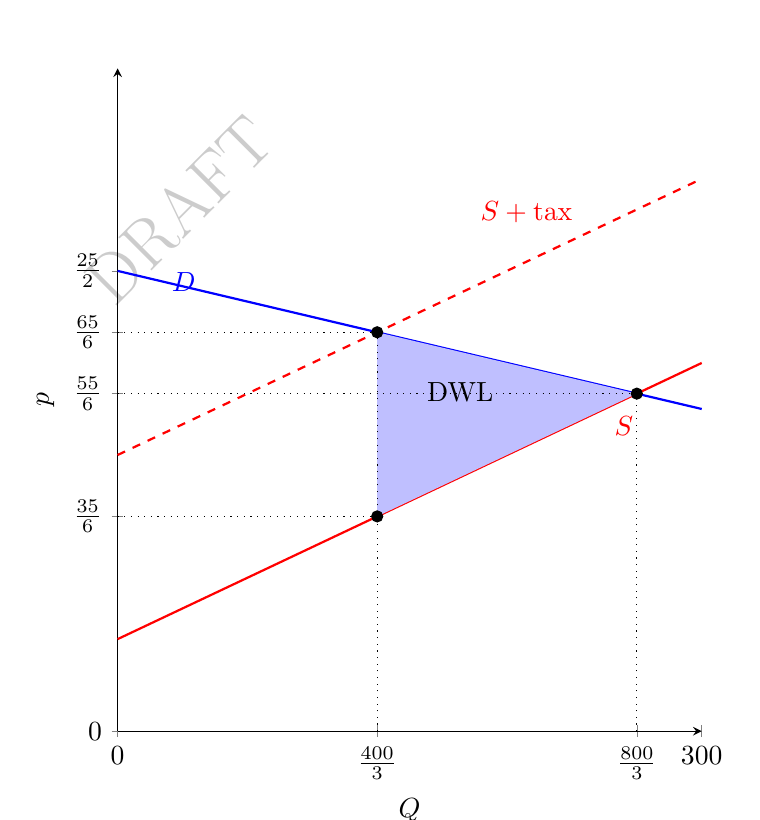
\begin{tikzpicture}
    \begin{axis}[
        width=9cm,
        height=10cm,
        xmin=0,xmax=300,
        ymin=0,ymax=18,
        axis lines=left,
        xlabel={$Q$},
        ylabel={$p$},
        xtick={0,133.3333,266.6667,300},
        xticklabels={$0$,$\frac{400}{3}$,$\frac{800}{3}$,$300$},
        ytick={0,5.8333,9.1667,10.8333,12.5},
        yticklabels={$0$,$\frac{35}{6}$,$\frac{55}{6}$,$\frac{65}{6}$,$\frac{25}{2}$},
        clip=false
    ]
    \addplot[thick,blue,domain=0:300,samples=2] {12.5 - x/80};
    \addplot[thick,red,domain=0:300,samples=2] {2.5 + x/40};
    \addplot[thick,red,dashed,domain=0:300,samples=2] {7.5 + x/40};

    \addplot[fill=blue!25,draw=none]
        coordinates {(133.3333,5.8333) (133.3333,10.8333) (266.6667,9.1667) (133.3333,5.8333)};

    \addplot[dotted] coordinates {(266.6667,0) (266.6667,9.1667)};
    \addplot[dotted] coordinates {(133.3333,0) (133.3333,10.8333)};
    \addplot[dotted] coordinates {(0,9.1667) (266.6667,9.1667)};
    \addplot[dotted] coordinates {(0,10.8333) (133.3333,10.8333)};
    \addplot[dotted] coordinates {(0,5.8333) (133.3333,5.8333)};

    \addplot[only marks,mark=*,mark size=2pt]
        coordinates {(266.6667,9.1667) (133.3333,10.8333) (133.3333,5.8333)};

    \node[blue] at (axis cs:34,12.2) {$D$};
    \node[red] at (axis cs:260,8.3) {$S$};
    \node[red] at (axis cs:210,14.1) {$S+\text{tax}$};
    \node at (axis cs:176,9.2) {DWL};
    \end{axis}
    \end{tikzpicture}
    \end{center}

    \item
    For general \(n\), before tax:
    \[
    1000-80p=4np-10n.
    \]
    So
    \[
    1000+10n=(80+4n)p
    \quad\Longrightarrow\quad
    p^*(n)=\frac{1000+10n}{80+4n}.
    \]
    The corresponding quantity is
    \[
    Q_0(n)=1000-80p^*(n)=\frac{800n}{n+20}.
    \]

    After a consumer tax of 5:
    \[
    p_b=p_s+5.
    \]
    Since
    \[
    Q_S=4np_s-10n,
    \]
    in terms of the buyers' price we have
    \[
    Q_S=4n(p_b-5)-10n=4np_b-30n.
    \]
    Equating with demand:
    \[
    1000-80p_b=4np_b-30n.
    \]
    Therefore
    \[
    1000+30n=(80+4n)p_b,
    \]
    and the taxed quantity is
    \[
    Q_t(n)=1000-80p_b=\frac{400n}{n+20}.
    \]

    Thus
    \[
    DWL(n)=\frac12\cdot 5\bigl(Q_0(n)-Q_t(n)\bigr)
    =\frac12\cdot 5\left(\frac{800n}{n+20}-\frac{400n}{n+20}\right).
    \]
    Hence
    \[
    \boxed{DWL(n)=\frac{1000n}{n+20}.}
    \]

    \item
    Since
    \[
    DWL(n)=\frac{1000n}{n+20},
    \]
    we differentiate:
    \[
    \frac{d}{dn}DWL(n)=\frac{20000}{(n+20)^2}>0.
    \]
    Therefore deadweight loss increases with the number of producers. Moreover,
    \[
    \lim_{n\to\infty}DWL(n)=1000.
    \]
    So
    \[
    \boxed{\text{DWL increases with }n\text{ and tends to }1000\text{ as }n\to\infty.}
    \]

    Intuitively, more firms make aggregate supply more elastic, so a given tax causes a larger quantity distortion and therefore a larger deadweight loss.
\end{enumerate}

\newpage
\subsubsection{Method 2: Inverse-demand / inverse-supply and welfare geometry}

\begin{enumerate}[label=(\alph*)]
    \item
    Since
    \[
    Q_S=4np-10n,
    \]
    the inverse supply curve is
    \[
    p_S(Q)=\frac{Q+10n}{4n}=\frac{Q}{4n}+\frac52.
    \]
    Thus
    \[
    \boxed{Q_S(p)=4np-10n,\qquad p_S(Q)=\frac{Q}{4n}+\frac52.}
    \]

    \item
    Inverse demand is
    \[
    p_D(Q)=\frac{1000-Q}{80}=\frac{25}{2}-\frac{Q}{80}.
    \]
    For \(n=10\), inverse supply is
    \[
    p_S(Q)=\frac{Q}{40}+\frac52.
    \]
    Before tax:
    \[
    \frac{25}{2}-\frac{Q}{80}=\frac{Q}{40}+\frac52.
    \]
    Thus
    \[
    10=\frac{3Q}{80}
    \quad\Longrightarrow\quad
    Q^*=\frac{800}{3}.
    \]
    Then
    \[
    p^*=\frac{25}{2}-\frac{1}{80}\cdot \frac{800}{3}=\frac{55}{6}.
    \]

    With a consumer tax of 5, the buyers' supply curve shifts up by 5:
    \[
    p_{S,t}(Q)=\frac{Q}{40}+\frac{15}{2}.
    \]
    Equating with inverse demand:
    \[
    \frac{25}{2}-\frac{Q}{80}=\frac{Q}{40}+\frac{15}{2}.
    \]
    Therefore
    \[
    5=\frac{3Q}{80}
    \quad\Longrightarrow\quad
    Q_t=\frac{400}{3}.
    \]
    The buyers' price is
    \[
    p_b=\frac{25}{2}-\frac{1}{80}\cdot \frac{400}{3}=\frac{65}{6},
    \]
    and the sellers' price is
    \[
    p_s=p_b-5=\frac{35}{6}.
    \]

    Hence
    \[
    \boxed{Q^*=\frac{800}{3},\quad p^*=\frac{55}{6},\quad Q_t=\frac{400}{3},\quad p_b=\frac{65}{6},\quad p_s=\frac{35}{6}.}
    \]

    The deadweight loss is
    \[
    DWL=\frac12\cdot 5\left(\frac{800}{3}-\frac{400}{3}\right)=\frac{1000}{3}.
    \]
    Therefore
    \[
    \boxed{DWL=\frac{1000}{3}.}
    \]

    \item
    For general \(n\), inverse supply is
    \[
    p_S(Q)=\frac{Q}{4n}+\frac52,
    \]
    while inverse demand is
    \[
    p_D(Q)=\frac{25}{2}-\frac{Q}{80}.
    \]

    Before tax:
    \[
    \frac{25}{2}-\frac{Q}{80}=\frac{Q}{4n}+\frac52.
    \]
    Hence
    \[
    10=Q\left(\frac{1}{80}+\frac{1}{4n}\right)
    =Q\frac{n+20}{80n},
    \]
    so
    \[
    Q_0(n)=\frac{800n}{n+20}.
    \]

    With tax \(t=5\), buyer-side inverse supply is
    \[
    p_{S,t}(Q)=\frac{Q}{4n}+\frac{15}{2}.
    \]
    Therefore
    \[
    \frac{25}{2}-\frac{Q}{80}=\frac{Q}{4n}+\frac{15}{2}
    \quad\Longrightarrow\quad
    5=Q\frac{n+20}{80n},
    \]
    so
    \[
    Q_t(n)=\frac{400n}{n+20}.
    \]
    Hence
    \[
    DWL(n)=\frac12\cdot 5\left(Q_0(n)-Q_t(n)\right)
    =\frac12\cdot 5\cdot \frac{400n}{n+20}
    =\frac{1000n}{n+20}.
    \]
    Therefore
    \[
    \boxed{DWL(n)=\frac{1000n}{n+20}.}
    \]

    \item
    Since the inverse supply slope is
    \[
    \frac{dp_S}{dQ}=\frac{1}{4n},
    \]
    it becomes flatter as \(n\) rises. Thus supply becomes more elastic, the tax causes a larger reduction in quantity, and deadweight loss rises. Therefore
    \[
    \boxed{\text{More producers } \Rightarrow \text{ more elastic supply } \Rightarrow \text{ larger DWL}.}
    \]
\end{enumerate}

\newpage
\subsubsection{Method 3: Concise olympiad-style tax-parameter method}

\begin{enumerate}[label=(\alph*)]
    \item
    Market supply is
    \[
    \boxed{Q_S(p)=4np-10n.}
    \]
    Equivalently,
    \[
    \boxed{p_S(Q)=\frac{Q}{4n}+\frac52.}
    \]

    \item
    For \(n=10\), inverse demand and supply are
    \[
    p_D(Q)=\frac{25}{2}-\frac{Q}{80},
    \qquad
    p_S(Q)=\frac{Q}{40}+\frac52.
    \]
    Introduce a general consumer tax \(t\). Then buyer-side inverse supply becomes
    \[
    p_{S,t}(Q)=\frac{Q}{40}+\frac52+t.
    \]
    Equilibrium is defined by
    \[
    \frac{25}{2}-\frac{Q}{80}=\frac{Q}{40}+\frac52+t.
    \]
    Rearranging,
    \[
    10-t=\frac{3Q}{80}.
    \]
    So
    \[
    Q_t=\frac{80}{3}(10-t).
    \]
    Therefore:
    \[
    Q_0=\frac{80}{3}(10)=\frac{800}{3},
    \qquad
    Q_5=\frac{80}{3}(5)=\frac{400}{3}.
    \]
    Then
    \[
    p^*=\frac{25}{2}-\frac{1}{80}\cdot \frac{800}{3}=\frac{55}{6},
    \]
    \[
    p_b=\frac{25}{2}-\frac{1}{80}\cdot \frac{400}{3}=\frac{65}{6},
    \qquad
    p_s=p_b-5=\frac{35}{6}.
    \]
    Therefore
    \[
    \boxed{p^*=\frac{55}{6},\quad Q^*=\frac{800}{3},\quad p_b=\frac{65}{6},\quad p_s=\frac{35}{6},\quad Q_t=\frac{400}{3}.}
    \]
    The deadweight loss follows immediately:
    \[
    DWL=\frac12\cdot 5\left(\frac{800}{3}-\frac{400}{3}\right)=\frac{1000}{3}.
    \]
    Hence
    \[
    \boxed{DWL=\frac{1000}{3}.}
    \]

    \item
    For general \(n\), buyer-side inverse supply with tax \(t\) is
    \[
    p_{S,t}(Q)=\frac{Q}{4n}+\frac52+t.
    \]
    Equilibrium solves
    \[
    \frac{25}{2}-\frac{Q}{80}=\frac{Q}{4n}+\frac52+t.
    \]
    Hence
    \[
    10-t=Q\left(\frac{1}{80}+\frac{1}{4n}\right)
    =Q\frac{n+20}{80n}.
    \]
    So the equilibrium quantity under tax \(t\) is
    \[
    \boxed{Q_t(n)=\frac{80n(10-t)}{n+20}.}
    \]
    In particular,
    \[
    Q_0(n)=\frac{800n}{n+20},
    \qquad
    Q_5(n)=\frac{400n}{n+20}.
    \]
    Therefore
    \[
    DWL(n)=\frac12\cdot 5\left(Q_0(n)-Q_5(n)\right)
    =\frac12\cdot 5\cdot \frac{400n}{n+20}.
    \]
    Thus
    \[
    \boxed{DWL(n)=\frac{1000n}{n+20}.}
    \]

    \item
    The formula
    \[
    DWL(n)=\frac{1000n}{n+20}
    \]
    is increasing in \(n\), because
    \[
    \frac{d}{dn}DWL(n)=\frac{20000}{(n+20)^2}>0.
    \]
    So
    \[
    \boxed{\text{DWL increases with }n.}
    \]
    This method is structurally concise because one solves the whole tax family at once via the parameter \(t\), then specialises to \(t=0\) and \(t=5\).
\end{enumerate}

\newpage
\subsubsection{Marking scheme (30 marks)}

\begin{enumerate}[label=(\alph*)]
    \item \textbf{(5 marks)} Market supply curve
    \begin{itemize}
        \item 2 marks: Correct aggregation of the individual supply curves across \(n\) firms.
        \item 2 marks: Correct simplified market supply curve in terms of \(n\).
        \item 1 mark: Correct treatment of the economically relevant domain / interpretation of the supply curve.
    \end{itemize}

    \item \textbf{(9 marks)} Tax analysis for \(n=10\)
    \begin{itemize}
        \item 2 marks: Correct market supply curve for \(n=10\).
        \item 2 marks: Correct no-tax equilibrium analysis and/or correct identification of the no-tax market outcome.
        \item 2 marks: Correct treatment of the consumer tax wedge and post-tax equilibrium analysis.
        \item 2 marks: Correct deadweight welfare loss conclusion, including a correct explanation.
        \item 1 mark: Diagram clearly showing the relevant demand and supply curves, with and without tax, together with the relevant equilibrium information.
    \end{itemize}

    \item \textbf{(10 marks)} Deadweight welfare loss as a function of \(n\)
    \begin{itemize}
        \item 3 marks: Correct no-tax equilibrium analysis in terms of \(n\), or a correct general argument about the pre-tax market outcome.
        \item 3 marks: Correct post-tax equilibrium analysis in terms of \(n\), or a correct general argument about the post-tax market outcome.
        \item 3 marks: Correct derivation of deadweight welfare loss as a function of \(n\).
        \item 1 mark: Correct final simplified expression.
    \end{itemize}

    \item \textbf{(6 marks)} Comparative statics of deadweight welfare loss
    \begin{itemize}
        \item 2 marks: Correct statement of how deadweight welfare loss changes with the number of producers.
        \item 2 marks: Correct supporting reasoning using the shape / elasticity / position of market supply.
        \item 2 marks: Clear economic intuition connecting the number of producers to the quantity distortion and welfare loss.
    \end{itemize}
\end{enumerate}



\newpage
\part{Tutorial 9}
%====================================================
% SAMPLE QUESTION 1
%====================================================
\section{Sample Question 1: Iris and Joseph in a Pure Exchange Economy}

\subsection{Problem}
\begin{itemize}
    \item Consider a small exchange economy, with two consumers Iris and Joseph, and two goods \(X\) and \(Y\). Iris is endowed with 15 units of \(X\) and 3 units of \(Y\). Joseph is endowed with 5 units of \(X\) and 7 units of \(Y\).

    Iris has utility
    \[
    U_I(X,Y)=\min\{X,3Y\}
    \]
    while Joseph has utility
    \[
    U_J(X,Y)=XY.
    \]

    \begin{enumerate}[label=(\alph*)]
        \item Draw the Edgeworth box for this exchange economy as accurately as possible, indicating the endowment and drawing several indifference curves for Iris and Joseph.
        \item In the figure you have drawn in (a), draw the indifference curves through the endowment and indicate where a competitive equilibrium must lie.
        \item Is the allocation where Iris gets \((X=12,Y=4)\) while Joseph gets \((X=8,Y=6)\) a fair allocation? Explain.
        \item ``There always exists an initial endowment for Iris and Joseph where the allocation in the consequent competitive equilibrium is fair for any (standard) preferences of Iris and Joseph.'' True or False? Explain.
    \end{enumerate}
\end{itemize}

\newpage
\subsection{Solution}

\subsubsection{Method 1: Marshallian-demand and market-clearing method}

\begin{enumerate}[label=(\alph*)]
    \item
    Total endowment is
    \[
    (\bar X,\bar Y)=(15+5,\,3+7)=(20,10).
    \]
    Hence the Edgeworth box has width \(20\) and height \(10\).

    Iris has utility
    \[
    U_I(X_I,Y_I)=\min\{X_I,3Y_I\},
    \]
    so her indifference curves are L-shaped, with kinks on the line
    \[
    X_I=3Y_I.
    \]
    Joseph has utility
    \[
    U_J(X_J,Y_J)=X_JY_J,
    \]
    so his indifference curves are smooth, strictly convex hyperbolas drawn from Joseph's origin at the top-right corner.

    The endowment point in Iris coordinates is
    \[
    e=(15,3).
    \]

    Therefore the diagram in part (a) should contain:
    \begin{itemize}
        \item the Edgeworth box \([0,20]\times[0,10]\);
        \item Iris' origin at the bottom-left and Joseph's origin at the top-right;
        \item the endowment point \(e=(15,3)\);
        \item several L-shaped indifference curves for Iris;
        \item several hyperbolic indifference curves for Joseph.
    \end{itemize}

    \item
    Normalise \(P_Y=1\) and write \(P_X=p\).

    Iris' income is
    \[
    m_I=15p+3.
    \]
    Since Iris has perfect-complements preferences, she demands goods in the ratio \(X_I=3Y_I\). Writing \(Y_I=t\), we have \(X_I=3t\), so the budget constraint is
    \[
    3pt+t=15p+3.
    \]
    Hence
    \[
    t=\frac{15p+3}{3p+1},
    \]
    and therefore Iris' demand is
    \[
    X_I=\frac{3(15p+3)}{3p+1},\qquad
    Y_I=\frac{15p+3}{3p+1}.
    \]

    Joseph's income is
    \[
    m_J=5p+7.
    \]
    Since \(U_J(X_J,Y_J)=X_JY_J\) is Cobb--Douglas with equal exponents, Joseph spends half his income on each good:
    \[
    X_J=\frac{m_J}{2p}=\frac{5p+7}{2p},
    \qquad
    Y_J=\frac{m_J}{2}=\frac{5p+7}{2}.
    \]

    Market clearing in good \(Y\) gives
    \[
    \frac{15p+3}{3p+1}+\frac{5p+7}{2}=10.
    \]
    Rearranging,
    \[
    15p^2-4p-7=0.
    \]
    Thus
    \[
    p=\frac{2+\sqrt{109}}{15}>0.
    \]

    So the competitive-equilibrium price ratio is
    \[
    \frac{P_X}{P_Y}=\frac{2+\sqrt{109}}{15}.
    \]

    Substituting into Iris' demand:
    \[
    Y_I^*=\frac{37-\sqrt{109}}{6},
    \qquad
    X_I^*=3Y_I^*=\frac{37-\sqrt{109}}{2}.
    \]
    Hence the competitive equilibrium allocation is
    \[
    x^*=\left(\frac{37-\sqrt{109}}{2},\,\frac{37-\sqrt{109}}{6}\right)
    \approx (13.28,\,4.43)
    \]
    for Iris, and therefore
    \[
    \left(20-\frac{37-\sqrt{109}}{2},\,10-\frac{37-\sqrt{109}}{6}\right)
    =
    \left(\frac{3+\sqrt{109}}{2},\,\frac{23+\sqrt{109}}{6}\right)
    \approx (6.72,\,5.57)
    \]
    for Joseph.

    The indifference curve through the endowment for Iris is
    \[
    U_I(15,3)=\min\{15,9\}=9,
    \]
    so it is the L-shaped indifference curve with kink at
    \[
    (9,3).
    \]
    For Joseph, at the endowment his bundle is \((5,7)\), so
    \[
    U_J(5,7)=35.
    \]
    In Iris coordinates this indifference curve is
    \[
    (20-X_I)(10-Y_I)=35.
    \]

    Since any competitive equilibrium must be Pareto efficient, it must lie on the contract curve. Here the contract curve is the locus of Iris' kink points:
    \[
    X_I=3Y_I.
    \]
    Thus in the diagram for part (b), the competitive equilibrium must lie on this line at the point where a supporting price line through the endowment touches the efficient frontier.

    A suitable Edgeworth box is shown below.

    \begin{center}
    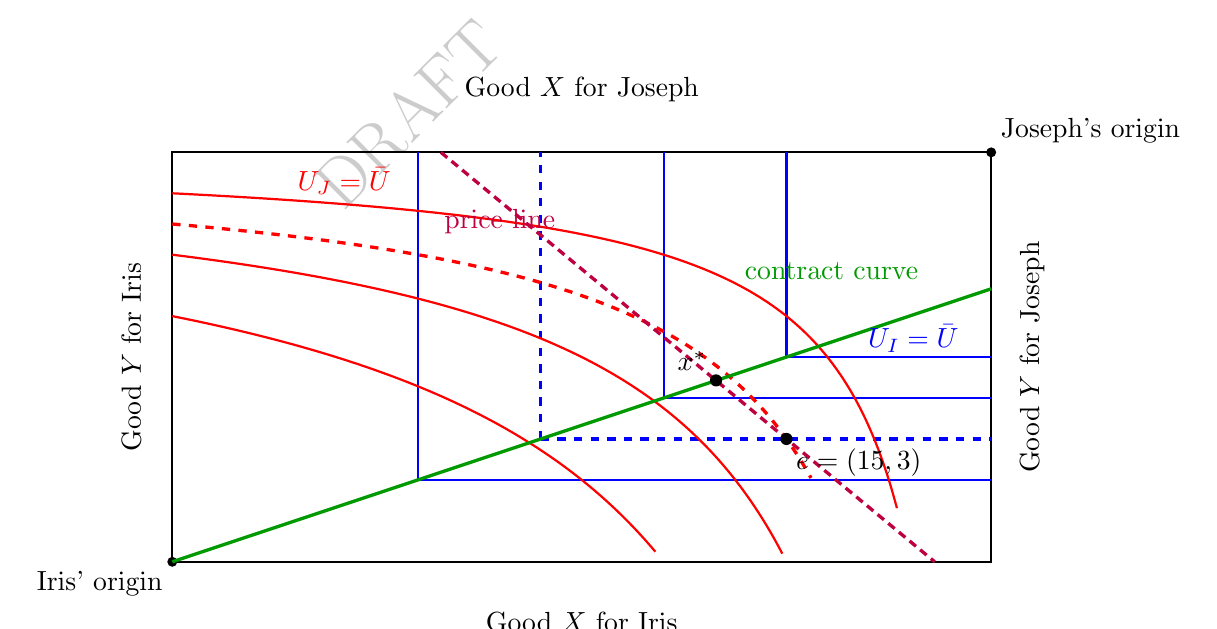
\begin{tikzpicture}[x=0.52cm,y=0.52cm]
      % Edgeworth box
      \draw[thick] (0,0) rectangle (20,10);

      % Origins
      \fill (0,0) circle (1.8pt);
      \fill (20,10) circle (1.8pt);
      \node[below left] at (0,0) {Iris' origin};
      \node[above right] at (20,10) {Joseph's origin};

      % Axis labels
      \node[below] at (10,-1.0) {Good \(X\) for Iris};
      \node[rotate=90] at (-1.0,5) {Good \(Y\) for Iris};
      \node[above] at (10,11.0) {Good \(X\) for Joseph};
      \node[rotate=90] at (21.0,5) {Good \(Y\) for Joseph};

      % Iris indifference curves
      \draw[blue, thick] (6,2) -- (6,10);
      \draw[blue, thick] (6,2) -- (20,2);

      \draw[blue, thick] (12,4) -- (12,10);
      \draw[blue, thick] (12,4) -- (20,4);

      \draw[blue, thick] (15,5) -- (15,10);
      \draw[blue, thick] (15,5) -- (20,5);

      % Iris indifference curve through endowment
      \draw[blue, dashed, very thick] (9,3) -- (9,10);
      \draw[blue, dashed, very thick] (9,3) -- (20,3);

      % Joseph indifference curves
      \draw[red, thick, domain=0:17.7, samples=120, smooth]
        plot (\x,{10-20/(20-\x)});
      \draw[red, thick, domain=0:14.9, samples=120, smooth]
        plot (\x,{10-50/(20-\x)});
      \draw[red, thick, domain=0:11.8, samples=120, smooth]
        plot (\x,{10-80/(20-\x)});

      % Joseph indifference curve through endowment
      \draw[red, dashed, very thick, domain=0:15.6, samples=120, smooth]
        plot (\x,{10-35/(20-\x)});

      % Contract curve
      \draw[green!60!black, very thick] (0,0) -- (20,6.6667);

      % Supporting line through endowment
      \draw[purple, densely dashed, very thick] (6.56,10) -- (18.62,0);

      % Endowment and CE
      \fill (15,3) circle (2.2pt) node[below right] {$e=(15,3)$};
      \fill (13.28,4.43) circle (2.2pt) node[above left] {$x^*$};

      % Labels
      \node[blue] at (18.1,5.45) {$U_I=\bar U$};
      \node[red] at (4.2,9.3) {$U_J=\bar U$};
      \node[green!60!black] at (16.1,7.1) {contract curve};
      \node[purple] at (8.0,8.3) {price line};
    \end{tikzpicture}
    \end{center}

\newpage
    \item
    Under the usual definition of fairness in exchange economies, namely envy-freeness, the proposed allocation is fair if neither consumer prefers the other's bundle to his or her own.

    At the proposed allocation,
    \[
    \text{Iris gets }(12,4),\qquad \text{Joseph gets }(8,6).
    \]

    Iris' utility from her own bundle is
    \[
    U_I(12,4)=\min\{12,12\}=12.
    \]
    If Iris were given Joseph's bundle instead, her utility would be
    \[
    U_I(8,6)=\min\{8,18\}=8.
    \]
    Hence Iris does not envy Joseph.

    Joseph's utility from his own bundle is
    \[
    U_J(8,6)=48.
    \]
    If Joseph were given Iris' bundle instead, his utility would be
    \[
    U_J(12,4)=48.
    \]
    So Joseph is indifferent between the two bundles and therefore does not envy Iris.

    The allocation is also feasible because
    \[
    (12+8,\,4+6)=(20,10).
    \]

    Hence the allocation is envy-free and feasible, so it is fair.

    \item
    The statement is \textbf{True}, under the standard assumptions used for competitive-equilibrium existence.

    A clean argument is to choose the \emph{equal division} of the aggregate endowment as the initial endowment:
    \[
    \omega_I=\omega_J=(10,5).
    \]
    Then both consumers have the same wealth at any given price vector.

    In any competitive equilibrium arising from this equal initial endowment, suppose Iris preferred Joseph's equilibrium bundle to her own. Since both bundles have the same equilibrium value and Iris could afford Joseph's bundle, this would contradict utility maximisation by Iris at equilibrium prices. The same argument applies to Joseph.

    Therefore any competitive equilibrium from an equal division of the aggregate endowment is envy-free, hence fair.

    So for any standard preferences for which a competitive equilibrium exists, there does exist an initial endowment---namely the equal division of the aggregate endowment---such that the consequent competitive equilibrium allocation is fair.
\end{enumerate}

\newpage
\subsubsection{Method 2: Contract-curve parameterisation method}

\begin{enumerate}[label=(\alph*)]
    \item
    Since the total endowment is
    \[
    (20,10),
    \]
    the Edgeworth box is again \([0,20]\times[0,10]\).

    Iris has Leontief-type preferences
    \[
    U_I(X_I,Y_I)=\min\{X_I,3Y_I\},
    \]
    so her indifference curves are L-shaped with kinks on
    \[
    X_I=3Y_I.
    \]
    Joseph's indifference curves are hyperbolas from the opposite origin because
    \[
    U_J(X_J,Y_J)=X_JY_J.
    \]
    The endowment point is
    \[
    e=(15,3).
    \]

    \item
    The key observation is that at any efficient allocation Iris must be at a kink:
    \[
    X_I=3Y_I.
    \]
    Hence efficient candidate allocations can be parameterised as
    \[
    (X_I,Y_I)=(3t,t),
    \qquad 0\le t\le \frac{20}{3}.
    \]
    Then Joseph receives
    \[
    (X_J,Y_J)=(20-3t,\,10-t).
    \]

    At a smooth point of Joseph's indifference curve, the supporting price ratio must satisfy
    \[
    \frac{P_X}{P_Y}=MRS_J=\frac{MU_X}{MU_Y}
    =\frac{Y_J}{X_J}
    =\frac{10-t}{20-3t}.
    \]
    Writing \(P_Y=1\) and \(P_X=p\), we therefore have
    \[
    p=\frac{10-t}{20-3t}.
    \]

    Since the equilibrium allocation must lie on the budget line through the endowment \(e=(15,3)\), Iris' bundle \((3t,t)\) must satisfy
    \[
    3pt+t=15p+3.
    \]
    Substituting
    \[
    p=\frac{10-t}{20-3t}
    \]
    into this equation yields
    \[
    3t^2-37t+105=0.
    \]
    Hence
    \[
    t=\frac{37\pm \sqrt{109}}{6}.
    \]
    The larger root is infeasible because it would imply \(3t>20\). Thus
    \[
    t=\frac{37-\sqrt{109}}{6}.
    \]

    Therefore the competitive equilibrium allocation is
    \[
    (X_I^*,Y_I^*)=(3t,t)
    =
    \left(\frac{37-\sqrt{109}}{2},\,\frac{37-\sqrt{109}}{6}\right),
    \]
    which is the same point found in Method 1.

    The indifference curves through the endowment are:
    \[
    U_I(15,3)=9
    \quad\Longrightarrow\quad
    \text{Iris' endowment indifference curve has kink at }(9,3),
    \]
    and
    \[
    U_J(5,7)=35
    \quad\Longrightarrow\quad
    (20-X_I)(10-Y_I)=35
    \]
    for Joseph in Iris coordinates.

    Thus the competitive equilibrium must lie on the contract curve
    \[
    X_I=3Y_I
    \]
    at the point where the supporting price line through the endowment touches the efficient set.

    \item
    At the proposed allocation
    \[
    \text{Iris gets }(12,4),\qquad \text{Joseph gets }(8,6),
    \]
    Iris' utility is
    \[
    U_I(12,4)=\min\{12,12\}=12,
    \]
    while if she were given Joseph's bundle, her utility would be
    \[
    U_I(8,6)=\min\{8,18\}=8.
    \]
    So Iris strictly prefers her own bundle.

    Joseph's utility from his own bundle is
    \[
    U_J(8,6)=48,
    \]
    and from Iris' bundle it is
    \[
    U_J(12,4)=48.
    \]
    Thus Joseph is indifferent.

    Since the allocation is feasible and neither person envies the other, it is fair.

    \item
    The statement is \textbf{True}.

    The structural reason is that one may choose the initial endowment to be the equal division of total resources:
    \[
    \omega_I=\omega_J=(10,5).
    \]
    Then both consumers enter the market with equal wealth. In any competitive equilibrium from such an equal division, each agent's chosen equilibrium bundle is at least as good as any other affordable bundle. Since the other consumer's bundle has exactly the same value at equilibrium prices, neither agent can prefer the other's bundle.

    Hence the resulting competitive equilibrium is envy-free, and therefore fair.
\end{enumerate}

\newpage
\subsubsection{Method 3: Supporting-prices and envy-freeness theorem method}

\begin{enumerate}[label=(\alph*)]
    \item
    The Edgeworth box is determined by aggregate resources
    \[
    (\bar X,\bar Y)=(20,10).
    \]
    Iris' preferences generate right-angled indifference curves with corners on
    \[
    X_I=3Y_I,
    \]
    while Joseph's preferences generate smooth hyperbolas from Joseph's origin.

    The endowment is
    \[
    e=(15,3)
    \]
    in Iris coordinates.

    \item
    A competitive equilibrium must be both feasible and Pareto efficient. Since Iris only values bundles through the smaller of \(X_I\) and \(3Y_I\), any efficient allocation must place her at a kink, hence on
    \[
    X_I=3Y_I.
    \]
    So even before calculation, one knows that the competitive equilibrium must lie on this line.

    To recover the exact equilibrium, normalise \(P_Y=1\) and let \(P_X=p\). At any competitive equilibrium, Joseph's smooth indifference curve must be tangent to the common supporting price line, so
    \[
    p=\frac{Y_J}{X_J}.
    \]
    Using feasibility with
    \[
    (X_I,Y_I)=(3t,t)
    \quad\text{and}\quad
    (X_J,Y_J)=(20-3t,10-t),
    \]
    this gives
    \[
    p=\frac{10-t}{20-3t}.
    \]
    Since Iris' chosen bundle must lie on the budget line through the endowment,
    \[
    3pt+t=15p+3.
    \]
    Solving yields
    \[
    t=\frac{37-\sqrt{109}}{6},
    \]
    so
    \[
    x^*=
    \left(\frac{37-\sqrt{109}}{2},\,\frac{37-\sqrt{109}}{6}\right).
    \]

    The indifference curves through the endowment are obtained from
    \[
    U_I(15,3)=9
    \quad\text{and}\quad
    U_J(5,7)=35.
    \]
    Hence Iris' endowment indifference curve has kink at \((9,3)\), while Joseph's is
    \[
    (20-X_I)(10-Y_I)=35.
    \]

    \item
    Fairness is checked by envy-freeness.

    For Iris:
    \[
    U_I(12,4)=12,
    \qquad
    U_I(8,6)=8.
    \]
    So Iris does not envy Joseph.

    For Joseph:
    \[
    U_J(8,6)=48,
    \qquad
    U_J(12,4)=48.
    \]
    So Joseph is indifferent and does not envy Iris.

    Therefore the allocation is fair.

    \item
    The statement is \textbf{True}. A standard theorem states that a competitive equilibrium with equal incomes is envy-free. Therefore, if one chooses the initial endowment to split the aggregate resources equally between the two consumers, any competitive equilibrium that results is fair.

    In this economy the equal split is
    \[
    \omega_I=\omega_J=(10,5).
    \]
    Thus there always exists an initial endowment that yields a fair competitive equilibrium.
\end{enumerate}
\vspace{3cm}
\subsubsection{Marking scheme (30 marks)}

\begin{enumerate}[label=(\alph*)]
    \item \textbf{(6 marks)} Edgeworth box and indifference curves
    \begin{itemize}
        \item 1 mark: Correct total endowment and hence correct dimensions of the Edgeworth box, namely \((20,10)\).
        \item 1 mark: Correct placement of Iris' and Joseph's origins, together with the correct endowment point \(e=(15,3)\) in Iris coordinates.
        \item 2 marks: Correct depiction of Iris' indifference curves as L-shaped, with kinks on the line \(X_I=3Y_I\).
        \item 2 marks: Correct depiction of Joseph's indifference curves as smooth convex hyperbolas from Joseph's origin.
    \end{itemize}

\newpage
    \item \textbf{(10 marks)} Indifference curves through the endowment and competitive equilibrium location
    \begin{itemize}
        \item 2 marks: Correct utility level for Iris at the endowment and hence correct indifference curve through the endowment, namely \(U_I(15,3)=9\) with kink at \((9,3)\).
        \item 2 marks: Correct utility level for Joseph at the endowment and hence correct indifference curve through the endowment, namely \(U_J(5,7)=35\), or an equivalent correctly drawn curve.
        \item 2 marks: Correct identification that any competitive equilibrium must be Pareto efficient and therefore lie on the contract curve.
        \item 2 marks: Correct identification of the contract curve / efficient locus as \(X_I=3Y_I\), i.e. Iris must be at a kink.
        \item 2 marks: Correct indication of a supporting price line through the endowment and a correct equilibrium location on the contract curve; full credit also if the exact competitive-equilibrium allocation is correctly computed.
    \end{itemize}

    \item \textbf{(6 marks)} Fairness of the allocation \((12,4)\) for Iris and \((8,6)\) for Joseph
    \begin{itemize}
        \item 2 marks: Correct computation of Iris' utility from her own bundle and from Joseph's bundle, with the correct conclusion that Iris does not envy Joseph.
        \item 2 marks: Correct computation of Joseph's utility from his own bundle and from Iris' bundle, with the correct conclusion that Joseph is indifferent and hence does not envy Iris.
        \item 1 mark: Correct verification of feasibility.
        \item 1 mark: Correct final conclusion that the allocation is fair under the envy-free interpretation.
    \end{itemize}

    \item \textbf{(8 marks)} Existence of an initial endowment yielding a fair competitive equilibrium
    \begin{itemize}
        \item 2 marks: Correct statement that the claim is \textbf{True}.
        \item 3 marks: Correct construction or explanation using equal division of the aggregate endowment, or an equivalent equal-income argument.
        \item 2 marks: Correct use of the competitive-equilibrium / equal-income intuition that each consumer weakly prefers his or her own equilibrium bundle to the other's bundle, so the equilibrium is envy-free.
        \item 1 mark: Clear final conclusion that there always exists such an initial endowment under standard assumptions.
    \end{itemize}
\end{enumerate}
%====================================================
% SAMPLE QUESTION 2
%====================================================
\newpage
\section{Sample Question 2: Leontief and Cobb--Douglas in a Pure Exchange Economy}

\subsection{Problem}
\begin{itemize}
    \item Consider the following two-good, two-person exchange economy.

    Person A has an endowment of 5 units of good \(X\) and 10 units of good \(Y\). He has preferences
    \[
    U_A(X,Y)=\min(X,Y).
    \]

    Person B has an endowment of 10 units of good \(X\) and 5 units of good \(Y\). He has preferences
    \[
    U_B(X,Y)=X^{0.4}Y^{0.6}.
    \]

    \begin{enumerate}[label=(\alph*)]
        \item Calculate the competitive equilibrium prices and allocations. You can assume that \(P_Y=1\).
        \item In an Edgeworth Box with Person A at the bottom left, Person B on the top right, good \(X\) on the \(x\)-axis and good \(Y\) on the \(y\)-axis, indicate the endowment and illustrate the competitive equilibrium of this economy.
    \end{enumerate}

    Let \((a,b)\) denote the feasible allocation where Person A receives \(a\) units of good \(X\) and \(b\) units of good \(Y\). This implies that Person B receives \(15-a\) units of good \(X\) and \(15-b\) units of good \(Y\).

    \begin{enumerate}[label=(\alph*),resume]
        \item Consider the feasible allocation \((7,7)\). Show that this is Pareto efficient and provide an endowment different from \((7,7)\) which will result in it being a competitive equilibrium after trading.
        \item ``For any exchange economy, the competitive equilibrium after trading will also be fair.'' True or False? Explain.
    \end{enumerate}
\end{itemize}

\newpage
\subsection{Solution}

\subsubsection{Method 1: Marshallian-demand and market-clearing method}

\begin{enumerate}[label=(\alph*)]
    \item
    Total endowment is
    \[
    (\bar X,\bar Y)=(5+10,\,10+5)=(15,15).
    \]

    Normalise \(P_Y=1\) and write \(P_X=p\).

    Person A has income
    \[
    m_A=5p+10.
    \]
    Since
    \[
    U_A(X,Y)=\min(X,Y),
    \]
    A chooses equal quantities of the two goods:
    \[
    X_A=Y_A=t.
    \]
    Using the budget constraint,
    \[
    pt+t=m_A=5p+10,
    \]
    so
    \[
    t=\frac{5p+10}{p+1}.
    \]
    Therefore
    \[
    X_A=Y_A=\frac{5p+10}{p+1}.
    \]

    Person B has income
    \[
    m_B=10p+5.
    \]
    Since B has Cobb--Douglas utility \(X^{0.4}Y^{0.6}\), the Marshallian demands are
    \[
    X_B=0.4\frac{m_B}{p},
    \qquad
    Y_B=0.6m_B.
    \]
    Hence
    \[
    X_B=0.4\frac{10p+5}{p},
    \qquad
    Y_B=0.6(10p+5).
    \]

    Market clearing in good \(X\) gives
    \[
    \frac{5p+10}{p+1}+0.4\frac{10p+5}{p}=15.
    \]
    Simplifying,
    \[
    \frac{5p+10}{p+1}+4+\frac{2}{p}=15,
    \]
    so
    \[
    \frac{5p+10}{p+1}+\frac{2}{p}=11.
    \]
    Multiply through by \(p(p+1)\):
    \[
    p(5p+10)+2(p+1)=11p(p+1).
    \]
    Therefore
    \[
    5p^2+10p+2p+2=11p^2+11p,
    \]
    hence
    \[
    6p^2-p-2=0.
    \]
    So
    \[
    p=\frac{1\pm 7}{12}.
    \]
    Since price must be positive,
    \[
    p=\frac23.
    \]

    Therefore the competitive-equilibrium prices are
    \[
    (P_X,P_Y)=\left(\frac23,1\right).
    \]

    Substituting back,
    \[
    m_A=5\cdot\frac23+10=\frac{40}{3},
    \]
    so
    \[
    X_A=Y_A=\frac{40/3}{5/3}=8.
    \]
    Thus
    \[
    (X_A,Y_A)=(8,8).
    \]

    Similarly,
    \[
    m_B=10\cdot\frac23+5=\frac{35}{3},
    \]
    and
    \[
    X_B=0.4\cdot\frac{35/3}{2/3}=7,
    \qquad
    Y_B=0.6\cdot\frac{35}{3}=7.
    \]
    Hence
    \[
    (X_B,Y_B)=(7,7).
    \]

    So the competitive equilibrium allocation is
    \[
    A:(8,8),\qquad B:(7,7).
    \]
\newpage
    \item
    The Edgeworth box has width \(15\) and height \(15\). The endowment point is
    \[
    e=(5,10)
    \]
    in A-coordinates, and the competitive equilibrium is
    \[
    x^*=(8,8)
    \]
    for A, equivalently \((7,7)\) for B.

    A's indifference curves are L-shaped with kinks on
    \[
    X_A=Y_A,
    \]
    while B's indifference curves are smooth and convex from B's origin at the top-right.

    A suitable Edgeworth box is shown below.

    \begin{center}
    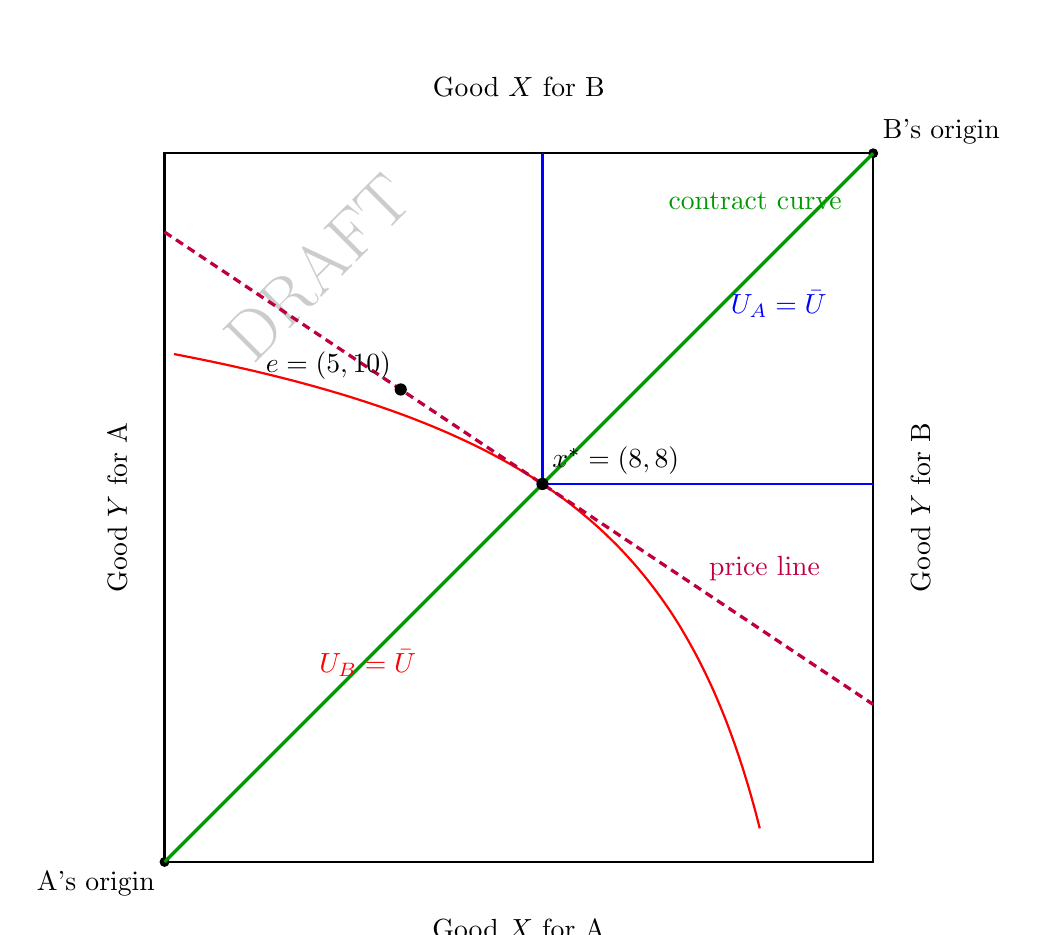
\begin{tikzpicture}[x=0.60cm,y=0.60cm]
      % Edgeworth box
      \draw[thick] (0,0) rectangle (15,15);

      % Origins
      \fill (0,0) circle (1.8pt);
      \fill (15,15) circle (1.8pt);
      \node[below left] at (0,0) {A's origin};
      \node[above right] at (15,15) {B's origin};

      % Axis labels
      \node[below] at (7.5,-1.0) {Good \(X\) for A};
      \node[rotate=90] at (-1.0,7.5) {Good \(Y\) for A};
      \node[above] at (7.5,16.0) {Good \(X\) for B};
      \node[rotate=90] at (16.0,7.5) {Good \(Y\) for B};

      % A indifference curve
      \draw[blue, thick] (8,8) -- (8,15);
      \draw[blue, thick] (8,8) -- (15,8);

      % B indifference curve through equilibrium
      \draw[red, thick, domain=0.2:12.6, samples=140, smooth]
        plot (\x,{15-((7)/((15-\x)^0.4))^(1/0.6)});

      % Contract curve
      \draw[green!60!black, very thick] (0,0) -- (15,15);

      % Budget line
      \draw[purple, densely dashed, very thick] (0,13.333) -- (15,3.333);

      % Endowment and equilibrium
      \fill (5,10) circle (2.2pt) node[above left] {$e=(5,10)$};
      \fill (8,8) circle (2.2pt) node[above right] {$x^*=(8,8)$};

      % Labels
      \node[blue] at (13.0,11.8) {$U_A=\bar U$};
      \node[red] at (4.3,4.2) {$U_B=\bar U$};
      \node[green!60!black] at (12.5,14.0) {contract curve};
      \node[purple] at (12.7,6.2) {price line};
    \end{tikzpicture}
    \end{center}

\newpage
    \item
    At the feasible allocation \((7,7)\), A receives
    \[
    (7,7)
    \]
    and B receives
    \[
    (8,8).
    \]

    To show Pareto efficiency, use supporting prices. At B's bundle \((8,8)\),
    \[
    MRS_B=\frac{MU_X}{MU_Y}
    =\frac{0.4X_B^{-0.6}Y_B^{0.6}}{0.6X_B^{0.4}Y_B^{-0.4}}
    =\frac{0.4}{0.6}\frac{Y_B}{X_B}
    =\frac23.
    \]
    So the supporting price ratio is
    \[
    \frac{P_X}{P_Y}=\frac23.
    \]

    At A's bundle \((7,7)\), A is exactly at the kink of the Leontief indifference curve \(X_A=Y_A\), so this same price ratio can support A's optimum. Therefore there exists a common supporting price vector, and hence \((7,7)\) is Pareto efficient.

    To produce \((7,7)\) as a competitive equilibrium after trade, choose an initial endowment for A that is different from \((7,7)\) but lies on the same budget line through \((7,7)\) at prices \(\left(\frac23,1\right)\). For example, take
    \[
    \omega_A'=(4,9).
    \]
    Then B's endowment is
    \[
    \omega_B'=(11,6).
    \]
    Check the value of A's endowment:
    \[
    \frac23\cdot 4+9=\frac{35}{3}.
    \]
    The value of A's target bundle \((7,7)\) is
    \[
    \frac23\cdot 7+7=\frac{35}{3}.
    \]
    So A can afford \((7,7)\), and similarly B can afford \((8,8)\). Hence with the endowment profile
    \[
    \omega_A'=(4,9),\qquad \omega_B'=(11,6),
    \]
    the allocation
    \[
    A:(7,7),\qquad B:(8,8)
    \]
    is a competitive equilibrium after trading.
\newpage
    \item
    The statement is \textbf{False}.

    Competitive equilibrium guarantees Pareto efficiency under standard assumptions, but it does \emph{not} guarantee fairness or envy-freeness for arbitrary initial endowments.

    A concrete counterexample can be built in this very economy. Suppose A initially owns everything:
    \[
    \omega_A=(15,15),\qquad \omega_B=(0,0).
    \]
    Take prices
    \[
    (P_X,P_Y)=(1,1).
    \]
    Then A's income is \(30\), and since A has utility \(\min(X,Y)\), A chooses
    \[
    (15,15).
    \]
    B has zero income and therefore chooses
    \[
    (0,0).
    \]
    Thus no trade is a competitive equilibrium.

    But this allocation is not fair, because B strictly prefers A's bundle:
    \[
    U_B(15,15)>U_B(0,0).
    \]
    Hence competitive equilibrium need not be fair.
\end{enumerate}

\newpage
\subsubsection{Method 2: Contract-curve and supporting-price method}

\begin{enumerate}[label=(\alph*)]
    \item
    Since
    \[
    U_A(X,Y)=\min(X,Y),
    \]
    any efficient allocation must put A at a kink:
    \[
    X_A=Y_A.
    \]
    So write
    \[
    (X_A,Y_A)=(t,t).
    \]
    By feasibility, B then receives
    \[
    (X_B,Y_B)=(15-t,15-t).
    \]

    At B's bundle, the Cobb--Douglas marginal rate of substitution is
    \[
    MRS_B=\frac{0.4}{0.6}\frac{Y_B}{X_B}
    =\frac{0.4}{0.6}\cdot 1
    =\frac23.
    \]
    Hence any interior supporting price vector must satisfy
    \[
    \frac{P_X}{P_Y}=\frac23.
    \]
    Normalising \(P_Y=1\), we get
    \[
    P_X=\frac23.
    \]

    A's income at the initial endowment \((5,10)\) is
    \[
    m_A=5\cdot\frac23+10=\frac{40}{3}.
    \]
    Since A chooses equal quantities,
    \[
    \frac23 t+t=\frac{40}{3}.
    \]
    Hence
    \[
    \frac53 t=\frac{40}{3}
    \quad\Longrightarrow\quad
    t=8.
    \]

    Therefore the competitive equilibrium allocation is
    \[
    A:(8,8),\qquad B:(7,7),
    \]
    with prices
    \[
    \left(\frac23,1\right).
    \]

    \item
    In the Edgeworth box, the endowment is
    \[
    e=(5,10),
    \]
    and the equilibrium is
    \[
    x^*=(8,8).
    \]
    The contract curve is the diagonal
    \[
    X_A=Y_A,
    \]
    because A must be at a kink at any efficient allocation and total resources of the two goods are equal.

    Hence the correct diagram has:
    \begin{itemize}
        \item the \(15\times 15\) Edgeworth box;
        \item A's origin at the bottom-left and B's origin at the top-right;
        \item the endowment \(e=(5,10)\);
        \item the equilibrium point \(x^*=(8,8)\);
        \item A's L-shaped indifference curve through \((8,8)\);
        \item B's smooth indifference curve through \((7,7)\) from B's origin;
        \item a supporting price line of slope \(-\frac23\) through the endowment and equilibrium.
    \end{itemize}

    \item
    For the allocation \((7,7)\), A gets \((7,7)\) and B gets \((8,8)\).

    A is exactly at a Leontief kink. At B's bundle,
    \[
    MRS_B=\frac23.
    \]
    Hence the price ratio
    \[
    \frac{P_X}{P_Y}=\frac23
    \]
    supports B's optimum and is also consistent with A being at a kink. Therefore \((7,7)\) is Pareto efficient.

    To make \((7,7)\) arise as a competitive equilibrium after trade, pick any different endowment for A on the same budget line through \((7,7)\). For instance,
    \[
    \omega_A'=(4,9),
    \qquad
    \omega_B'=(11,6).
    \]
    At prices \(\left(\frac23,1\right)\), \((7,7)\) has the same value as \((4,9)\), so the target allocation is supported.

    \item
    The statement is \textbf{False}. Efficiency does not imply fairness.

    In this same economy, if A owns all resources initially,
    \[
    \omega_A=(15,15),\qquad \omega_B=(0,0),
    \]
    then a no-trade competitive equilibrium exists, but B envies A. So a competitive equilibrium need not be fair.
\end{enumerate}

\newpage
\subsubsection{Method 3: Expenditure-share and counterexample method}

\begin{enumerate}[label=(\alph*)]
    \item
    Let \(P_Y=1\) and \(P_X=p\).

    A always chooses equal quantities because
    \[
    U_A(X,Y)=\min(X,Y).
    \]
    Hence A's demand must take the form
    \[
    (X_A,Y_A)=(t,t).
    \]
    Since A's income is \(5p+10\), this gives
    \[
    pt+t=5p+10
    \quad\Longrightarrow\quad
    t=\frac{5p+10}{p+1}.
    \]

    B has Cobb--Douglas utility \(X^{0.4}Y^{0.6}\), so B spends \(40\%\) of income on \(X\) and \(60\%\) on \(Y\). Therefore,
    \[
    X_B=0.4\frac{10p+5}{p},
    \qquad
    Y_B=0.6(10p+5).
    \]

    Using one market-clearing equation,
    \[
    \frac{5p+10}{p+1}+0.4\frac{10p+5}{p}=15,
    \]
    which simplifies to
    \[
    6p^2-p-2=0.
    \]
    Hence
    \[
    p=\frac23.
    \]
    Substituting gives
    \[
    A:(8,8),\qquad B:(7,7).
    \]

    \item
    The Edgeworth-box picture is then immediate:
    \begin{itemize}
        \item total resources are \((15,15)\), so the box is \(15\times 15\);
        \item the endowment is \(e=(5,10)\);
        \item the competitive equilibrium is \(x^*=(8,8)\) for A;
        \item the price line has slope \(-\frac23\);
        \item the equilibrium lies on the diagonal \(X_A=Y_A\), which is the efficient locus generated by A's Leontief preferences.
    \end{itemize}
\newpage
    \item
    At allocation \((7,7)\), A's bundle is exactly balanced, so A is at a kink. B receives \((8,8)\), and at that bundle
    \[
    MRS_B=\frac{0.4}{0.6}\frac{8}{8}=\frac23.
    \]
    Therefore a supporting price line with slope \(-\frac23\) exists, so the allocation is Pareto efficient.

    A different endowment that supports this allocation is
    \[
    \omega_A'=(4,9),
    \qquad
    \omega_B'=(11,6).
    \]
    At prices \(\left(\frac23,1\right)\), both consumers can afford their target bundles, and these bundles are utility-maximising, so the target allocation is a competitive equilibrium after trade.

    \item
    The statement is \textbf{False}. A competitive equilibrium can be efficient but highly unequal.

    For example, if
    \[
    \omega_A=(15,15),\qquad \omega_B=(0,0),
    \]
    then no trade can be a competitive equilibrium, yet B envies A. Therefore competitive equilibrium after trade need not be fair in general.
\end{enumerate}

\newpage
\subsubsection{Marking scheme (30 marks)}

\begin{enumerate}[label=(\alph*)]
    \item \textbf{(10 marks)} Competitive equilibrium prices and allocations
    \begin{itemize}
        \item 2 marks: Correct incomes for A and B after normalising \(P_Y=1\) and writing \(P_X=p\).
        \item 2 marks: Correct demand for A using the Leontief structure \(X_A=Y_A\).
        \item 2 marks: Correct Marshallian demand for B using the Cobb--Douglas expenditure shares.
        \item 2 marks: Correct market-clearing equation and correct equilibrium price \(p=\frac23\).
        \item 2 marks: Correct equilibrium allocations \(A:(8,8)\) and \(B:(7,7)\).
    \end{itemize}

    \item \textbf{(6 marks)} Edgeworth-box illustration of the equilibrium
    \begin{itemize}
        \item 1 mark: Correct dimensions of the Edgeworth box, namely \((15,15)\).
        \item 1 mark: Correct endowment point \(e=(5,10)\) in A-coordinates.
        \item 1 mark: Correct equilibrium point \(x^*=(8,8)\) in A-coordinates.
        \item 1 mark: Correct depiction of A's indifference curves as L-shaped with kinks on \(X_A=Y_A\).
        \item 1 mark: Correct depiction of B's indifference curves as smooth convex curves from B's origin.
        \item 1 mark: Correct indication of the supporting price line and / or the contract curve through the equilibrium.
    \end{itemize}

    \item \textbf{(8 marks)} Pareto efficiency of \((7,7)\) and supporting endowment
    \begin{itemize}
        \item 2 marks: Correct identification of the implied bundle for B, namely \((8,8)\).
        \item 2 marks: Correct supporting-price or marginal-rate-of-substitution argument showing that \((7,7)\) is Pareto efficient.
        \item 2 marks: Correct construction of an endowment different from \((7,7)\) that lies on the supporting budget line through the target allocation, for example \((4,9)\) for A.
        \item 2 marks: Correct verification that the proposed endowment supports \((7,7)\) as a competitive equilibrium after trade, or an equivalent correct supporting argument.
    \end{itemize}

    \item \textbf{(6 marks)} Fairness of competitive equilibrium in general
    \begin{itemize}
        \item 2 marks: Correct statement that the claim is \textbf{False}.
        \item 2 marks: Correct explanation that competitive equilibrium guarantees Pareto efficiency, not fairness or envy-freeness in general.
        \item 2 marks: Correct counterexample or equivalent reasoning showing that a competitive equilibrium can be efficient but not fair.
    \end{itemize}
\end{enumerate}


\newpage
\part{Tutorial 10}
\section{Sample Question 1: Weighted Borda Voting}

\subsection{Problem}

There are three policies \(X,Y,Z\), and three preference types:

\[
\text{Young: } Z \succ Y \succ X,
\qquad
\text{Middle Aged: } X \succ Z \succ Y,
\qquad
\text{Old: } Y \succ X \succ Z.
\]

The numbers of voters are:
\[
300 \text{ young}, \qquad 300 \text{ middle aged}, \qquad 400 \text{ old}.
\]

Under \emph{standard Borda voting} with three alternatives, each voter awards:
\[
\text{1st place } = 2 \text{ points}, 
\qquad
\text{2nd place } = 1 \text{ point}, 
\qquad
\text{3rd place } = 0 \text{ points}.
\]

Under the \emph{modified Borda voting} rule, the same ranking scores apply, except:
\begin{itemize}[leftmargin=*]
    \item young voters' points are multiplied by \(2\),
    \item middle-aged voters' points are multiplied by \(1.5\),
    \item old voters' points remain unchanged.
\end{itemize}

\begin{enumerate}[label=(\alph*)]
    \item In general, would the modified Borda voting rule make the social decision tend to align more with the old, the middle-aged, or the young? Explain briefly.
    \item Does the modified Borda voting rule satisfy the Pareto condition? Explain briefly.
    \item Which policy would be chosen under the standard Borda voting rule, and which policy would be chosen under the modified Borda voting rule?
    \item Do you think the modified Borda voting rule is more reasonable in this environmental policy context? Briefly explain.
\end{enumerate}

\newpage

\subsection{Solution}

\subsubsection{Method 1: Direct weighted-score computation}

\begin{enumerate}[label=(\alph*)]
    \item
    In general, the modified Borda rule gives more weight to the preferences of young and middle-aged consumers relative to old consumers.

    Under standard Borda, each person's ranking contributes equally. Under the modified rule:
    \[
    \text{Young weight }=2,
    \qquad
    \text{Middle-aged weight }=1.5,
    \qquad
    \text{Old weight }=1.
    \]
    So the social ranking will tend to shift toward alternatives that are ranked highly by the young and middle-aged groups, and away from alternatives that are mainly supported by the old group.

    In this problem:
    \begin{itemize}[leftmargin=*]
        \item the young rank \(Z\) first,
        \item the middle-aged rank \(X\) first,
        \item the old rank \(Y\) first.
    \end{itemize}

    Hence, compared with standard Borda voting:
    \begin{itemize}[leftmargin=*]
        \item \(Z\) should gain because the young are heavily up-weighted,
        \item \(X\) should also gain because the middle-aged are up-weighted,
        \item \(Y\) is likely to lose relative ground because the old group is not up-weighted.
    \end{itemize}

    Therefore
    \[
    \boxed{\text{the modified rule tends to align more with the young and middle-aged, especially the young.}}
    \]

    \item
    Yes, the modified Borda voting rule satisfies the Pareto condition.

    If every individual strictly prefers policy \(A\) to policy \(B\), then under ordinary Borda scoring each person assigns strictly more points to \(A\) than to \(B\). Under the modified rule, these scores are multiplied by strictly positive weights \(2\), \(1.5\), and \(1\), so the strict inequality is preserved for every voter.

    Summing across all voters, the total weighted Borda score of \(A\) must exceed that of \(B\). Therefore the social ranking also places \(A\) above \(B\).

    Hence
    \[
    \boxed{\text{the modified Borda rule satisfies the Pareto condition.}}
    \]

    \item
    \textbf{Standard Borda voting.}

    The three groups rank:
    \[
    \text{Young: } Z \succ Y \succ X,
    \qquad
    \text{Middle Aged: } X \succ Z \succ Y,
    \qquad
    \text{Old: } Y \succ X \succ Z.
    \]

    Using the standard \(2,1,0\) scoring rule:
    \[
    \begin{aligned}
    \text{Score}(X)
    &=300(0)+300(2)+400(1)=1000,\\
    \text{Score}(Y)
    &=300(1)+300(0)+400(2)=1100,\\
    \text{Score}(Z)
    &=300(2)+300(1)+400(0)=900.
    \end{aligned}
    \]
    Therefore the standard Borda social ranking is
    \[
    Y \succ X \succ Z,
    \]
    so the chosen policy is
    \[
    \boxed{Y.}
    \]

    \bigskip

    \textbf{Modified Borda voting.}

    Under the modified rule:
    \begin{itemize}[leftmargin=*]
        \item young scores are multiplied by \(2\),
        \item middle-aged scores are multiplied by \(1.5\),
        \item old scores are unchanged.
    \end{itemize}

    So the weighted contributions are:
    \[
    \begin{aligned}
    \text{Modified Score}(X)
    &=300(0)(2)+300(2)(1.5)+400(1)(1)\\
    &=0+900+400=1300,\\
    \text{Modified Score}(Y)
    &=300(1)(2)+300(0)(1.5)+400(2)(1)\\
    &=600+0+800=1400,\\
    \text{Modified Score}(Z)
    &=300(2)(2)+300(1)(1.5)+400(0)(1)\\
    &=1200+450+0=1650.
    \end{aligned}
    \]
    Therefore the modified Borda social ranking is
    \[
    Z \succ Y \succ X,
    \]
    so the chosen policy is
    \[
    \boxed{Z.}
    \]

    Hence
    \[
    \boxed{\text{Standard Borda chooses }Y,\qquad \text{Modified Borda chooses }Z.}
    \]

    \item
    A reasonable argument in favour of the modified Borda rule is that environmental policy has long-term consequences, so it may be appropriate to give greater weight to groups who will live with those consequences for longer.

    In this scenario:
    \begin{itemize}[leftmargin=*]
        \item young consumers are likely to be affected by environmental outcomes over a longer remaining lifetime,
        \item middle-aged consumers also have substantial future exposure,
        \item old consumers may be affected for a shorter period.
    \end{itemize}

    Under standard Borda voting, each person has the same weight regardless of how long they will experience the effects of the policy. The modified rule instead places more emphasis on the preferences of those with a longer future stake.

    A criticism, however, is that it violates the principle of equal political weight or ``one person, one vote.'' So whether it is more reasonable depends on the ethical principle being used.

    A balanced conclusion is:
    \[
    \boxed{\text{The modified rule may be more reasonable if one believes voting power should reflect long-run stake in environmental outcomes, but less reasonable if one insists on equal weight for every voter.}}
    \]
\end{enumerate}

\subsubsection{Method 2: Linear-functional / vector method}

\begin{enumerate}[label=(\alph*)]
    \item
    Write the standard Borda score vector for \((\text{1st},\text{2nd},\text{3rd})\) as
    \[
    s=(2,1,0).
    \]
    The modified rule is simply a reweighting of group contributions by
    \[
    w=(2,1.5,1).
    \]
    Since the young and middle-aged groups are upweighted relative to the old group, the induced social ranking shifts toward the alternatives they rank highly. Since the young place \(Z\) first and the middle-aged place \(X\) first, while the old place \(Y\) first, the modified rule moves weight away from \(Y\) and toward \(Z\) and \(X\), especially \(Z\).

    \item
    The Pareto condition follows immediately from positivity of the weights. If every voter ranks \(A\) above \(B\), then every group contributes a strictly larger Borda score to \(A\) than to \(B\). Multiplying by positive weights preserves the inequality, so total weighted score still ranks \(A\) above \(B\).

    \item
    Let the score vector for each policy under the three groups be:
    \[
    X=(0,2,1),\qquad Y=(1,0,2),\qquad Z=(2,1,0).
    \]
    Under standard Borda, with population vector
    \[
    n=(300,300,400),
    \]
    the total scores are proportional to
    \[
    \langle n,X\rangle =1000,\qquad
    \langle n,Y\rangle =1100,\qquad
    \langle n,Z\rangle =900.
    \]
    Hence
    \[
    \boxed{Y \succ X \succ Z.}
    \]

    Under modified Borda, the effective population vector is
    \[
    n'=(600,450,400),
    \]
    so
    \[
    \langle n',X\rangle =1300,\qquad
    \langle n',Y\rangle =1400,\qquad
    \langle n',Z\rangle =1650.
    \]
    Hence
    \[
    \boxed{Z \succ Y \succ X.}
    \]

    Therefore standard Borda chooses \(Y\) and modified Borda chooses \(Z\).

    \item
    In this representation, the modified rule changes the social ranking by changing the weight vector. So the normative question is whether one regards this change of weight vector as ethically justified. If voting weight should reflect future stake, the modification is defensible; if all persons should count equally, it is not.
\end{enumerate}

\newpage
\subsubsection{Method 3: Pairwise score-difference method}

\begin{enumerate}[label=(\alph*)]
    \item
    Under the modified rule, the relative influence of the young and middle-aged groups rises, while the old group keeps weight 1. Therefore alternatives favoured by the young and middle-aged gain relative to alternatives favoured mainly by the old.

    \item
    If everyone ranks \(A\) above \(B\), then each individual contributes a strictly higher Borda score to \(A\) than to \(B\). Positive reweighting preserves this group-by-group advantage, so the aggregate ranking still has \(A\) above \(B\). Thus Pareto holds.

    \item
    Instead of computing all totals, compare relevant score differences.

    Under standard Borda:
    \[
    \begin{aligned}
    \text{Score}(Y)-\text{Score}(X)
    &=300(1-0)+300(0-2)+400(2-1)\\
    &=300-600+400=100>0,
    \end{aligned}
    \]
    so \(Y\succ X\).

    Also,
    \[
    \begin{aligned}
    \text{Score}(X)-\text{Score}(Z)
    &=300(0-2)+300(2-1)+400(1-0)\\
    &=-600+300+400=100>0,
    \end{aligned}
    \]
    so \(X\succ Z\). Hence
    \[
    \boxed{Y \succ X \succ Z.}
    \]

    Under modified Borda:
    \[
    \begin{aligned}
    \text{Score}(Z)-\text{Score}(Y)
    &=300\cdot 2(2-1)+300\cdot 1.5(1-0)+400\cdot 1(0-2)\\
    &=600+450-800=250>0,
    \end{aligned}
    \]
    so \(Z\succ Y\).

    Next,
    \[
    \begin{aligned}
    \text{Score}(Y)-\text{Score}(X)
    &=300\cdot 2(1-0)+300\cdot 1.5(0-2)+400\cdot 1(2-1)\\
    &=600-900+400=100>0,
    \end{aligned}
    \]
    so \(Y\succ X\). Hence
    \[
    \boxed{Z \succ Y \succ X.}
    \]

    \item
    Since the modified rule makes \(Z\) overtake \(Y\) precisely because of the heavier weight placed on the young and middle-aged, the reasonableness of the rule depends on whether that reweighting is normatively acceptable.
\end{enumerate}
\newpage\subsubsection{Marking scheme (20 marks)}

\begin{enumerate}[label=(\alph*)]
    \item \textbf{(4 marks)} Comparative effect of the modified weights
    \begin{itemize}[leftmargin=*]
        \item 2 marks: Correct identification that the modified rule shifts influence toward the young and middle-aged, especially the young.
        \item 2 marks: Clear explanation using the weight changes \(2,1.5,1\) and the ranking pattern of the three groups.
    \end{itemize}

    \item \textbf{(4 marks)} Pareto condition
    \begin{itemize}[leftmargin=*]
        \item 2 marks: Correct conclusion that the modified Borda rule satisfies the Pareto condition.
        \item 2 marks: Correct justification that positive weighting preserves the strict score advantage of a unanimously preferred alternative.
    \end{itemize}

    \item \textbf{(8 marks)} Policy choice under standard and modified Borda
    \begin{itemize}[leftmargin=*]
        \item 3 marks: Correct standard Borda score calculation or an equivalent correct derivation.
        \item 3 marks: Correct modified Borda score calculation or an equivalent correct derivation.
        \item 2 marks: Correct final conclusion that standard Borda chooses \(Y\) while modified Borda chooses \(Z\).
    \end{itemize}

    \item \textbf{(4 marks)} Reasonableness in context
    \begin{itemize}[leftmargin=*]
        \item 2 marks: A coherent argument in favour of the modified rule based on long-run stake / intergenerational exposure.
        \item 2 marks: Recognition of the counterargument concerning equal political weight, together with a balanced conclusion.
    \end{itemize}
\end{enumerate}
% ============================================================
% QUESTION 2
% ============================================================

\newpage
\section{Sample Question 2: Utility Possibility Frontier and Welfare Optimisation}

\subsection{Problem}

The utility possibility frontier (UPF) is given by
\[
U_I + U_J^2 = 10.
\]

We assume utilities are non-negative, so the relevant part of the frontier is
\[
U_I \ge 0,\qquad U_J \ge 0.
\]

\begin{enumerate}[label=(\alph*)]
    \item Explain what the utility possibility frontier means, and sketch it in the \((U_I,U_J)\)-plane.
    \item If a utilitarian social planner maximizes
    \[
    W(U_I,U_J)=U_I+U_J,
    \]
    what is the planner's ideal allocation?
    \item If a weighted-utilitarian social welfare function is used, and the planner's ideal allocation is
    \[
    U_I=1,\qquad U_J=3,
    \]
    what weighted-utilitarian social welfare function would support this point?
    \item Is every point on the utility possibility frontier necessarily obtainable as a competitive equilibrium? Briefly explain.
\end{enumerate}

\newpage
\subsection{Solution}

\subsubsection{Method 1: Direct substitution and tangency}

\begin{enumerate}[label=(\alph*)]
    \item
    The \emph{utility possibility frontier} is the boundary of all utility pairs \((U_I,U_J)\) that can be achieved in the economy when resources are allocated efficiently.

    In other words:
    \begin{itemize}[leftmargin=*]
        \item the feasible utility set consists of all utility pairs the economy can generate,
        \item the \emph{frontier} consists of the Pareto efficient utility pairs,
        \item at a point on the frontier, one person's utility can be increased only by decreasing the other person's utility.
    \end{itemize}

    Since
    \[
    U_I + U_J^2 = 10,
    \]
    we can write the frontier as
    \[
    U_I = 10 - U_J^2
    \]
    or equivalently
    \[
    U_J = \sqrt{10-U_I}.
    \]

    The intercepts are:
    \[
    U_J=0 \implies U_I=10,
    \qquad
    U_I=0 \implies U_J=\sqrt{10}.
    \]
    So the UPF is downward sloping and bowed toward the origin in the \((U_I,U_J)\)-diagram, and the feasible set is
    \[
    \boxed{U_I+U_J^2\le 10.}
    \]
    A suitable graph is:

    \begin{center}
    \begin{tikzpicture}
    \begin{axis}[
        width=11.5cm,
        height=8cm,
        xmin=0,xmax=10.5,
        ymin=0,ymax=3.6,
        axis lines=left,
        xlabel={$U_I$},
        ylabel={$U_J$},
        xtick={0,1,39/4,10},
        xticklabels={$0$,$1$,$\frac{39}{4}$,$10$},
        ytick={0,1/2,3,sqrt(10)},
        yticklabels={$0$,$\frac12$,$3$,$\sqrt{10}$},
        samples=200,
        domain=0:10,
        clip=false
    ]
    \addplot[thick,blue] {sqrt(10-x)};
    \addplot[dashed] coordinates {(1,0) (1,3)};
    \addplot[dashed] coordinates {(0,3) (1,3)};
    \addplot[dashed] coordinates {(39/4,0) (39/4,1/2)};
    \addplot[dashed] coordinates {(0,1/2) (39/4,1/2)};
    \addplot[only marks,mark=*,mark size=2pt] coordinates {(1,3) (39/4,1/2)};
    \node[blue] at (axis cs:7.9,2.1) {UPF: $U_J=\sqrt{10-U_I}$};
    \node at (axis cs:1.5,3.18) {$(1,3)$};
    \node at (axis cs:8.5,0.72) {$\left(\frac{39}{4},\frac12\right)$};
    \end{axis}
    \end{tikzpicture}
    \end{center}
    \item
    A utilitarian social planner maximizes
    \[
    W(U_I,U_J)=U_I+U_J.
    \]
    Since on the frontier
    \[
    U_I=10-U_J^2,
    \]
    substitute into welfare:
    \[
    W(U_J)=10-U_J^2+U_J.
    \]
    Differentiate:
    \[
    \frac{dW}{dU_J}=-2U_J+1.
    \]
    Set equal to zero:
    \[
    -2U_J+1=0
    \quad\Longrightarrow\quad
    U_J=\frac12.
    \]
    Then
    \[
    U_I=10-\left(\frac12\right)^2=10-\frac14=\frac{39}{4}.
    \]
    Therefore the utilitarian optimum is
    \[
    \boxed{U_I^*=\frac{39}{4},\qquad U_J^*=\frac12.}
    \]

    \item
    A weighted-utilitarian social welfare function has the form
    \[
    W(U_I,U_J)=\alpha U_I+\beta U_J,
    \qquad \alpha,\beta>0.
    \]
    We are told that the ideal allocation is
    \[
    U_I=1,\qquad U_J=3.
    \]
    First check feasibility:
    \[
    1+3^2=10.
    \]
    So the point lies on the frontier.

    Substitute \(U_I=10-U_J^2\) into welfare:
    \[
    W(U_J)=\alpha(10-U_J^2)+\beta U_J.
    \]
    Differentiate:
    \[
    \frac{dW}{dU_J}=-2\alpha U_J+\beta.
    \]
    Set equal to zero at \(U_J=3\):
    \[
    -2\alpha(3)+\beta=0
    \quad\Longrightarrow\quad
    \beta=6\alpha.
    \]
    So the required weight ratio is
    \[
    \boxed{\frac{\beta}{\alpha}=6.}
    \]
    One valid supporting welfare function is
    \[
    \boxed{W(U_I,U_J)=U_I+6U_J.}
    \]

    \item
    Not every point on the utility possibility frontier is necessarily obtainable as a competitive equilibrium from a \emph{given} initial endowment.

    The relevant economic principles are:
    \begin{itemize}[leftmargin=*]
        \item The \emph{First Welfare Theorem}: every competitive equilibrium allocation is Pareto efficient under the usual assumptions.
        \item The \emph{Second Welfare Theorem}: under suitable convexity assumptions, every Pareto efficient allocation can be decentralised as a competitive equilibrium for \emph{some} suitable redistribution of endowments.
    \end{itemize}

    Therefore:
    \[
    \boxed{\text{Not necessarily for a fixed endowment, but under the standard assumptions every point on the UPF can be supported as a competitive equilibrium for some suitable redistribution of endowments.}}
    \]
\end{enumerate}

\newpage
\subsubsection{Method 2: Lagrangian method}

\begin{enumerate}[label=(\alph*)]
    \item
    The UPF is the boundary of the feasible utility set
    \[
    \{(U_I,U_J)\in \R_+^2: U_I+U_J^2\le 10\}.
    \]
    The frontier itself is
    \[
    U_I+U_J^2=10,
    \]
    with intercepts \((10,0)\) and \((0,\sqrt{10})\).

    \item
    Maximize
    \[
    U_I+U_J
    \]
    subject to
    \[
    U_I+U_J^2=10.
    \]
    The Lagrangian is
    \[
    \mathcal L = U_I+U_J+\lambda(10-U_I-U_J^2).
    \]
    First-order conditions:
    \begin{align*}
        \frac{\partial \mathcal L}{\partial U_I} &= 1-\lambda=0,\\
        \frac{\partial \mathcal L}{\partial U_J} &= 1-2\lambda U_J=0.
    \end{align*}
    From the first equation,
    \[
    \lambda=1.
    \]
    Substitute into the second:
    \[
    1-2U_J=0
    \quad\Longrightarrow\quad
    U_J=\frac12.
    \]
    Then
    \[
    U_I=10-\left(\frac12\right)^2=\frac{39}{4}.
    \]
    Hence
    \[
    \boxed{\left(U_I^*,U_J^*\right)=\left(\frac{39}{4},\frac12\right).}
    \]
\newpage
    \item
    Now maximize
    \[
    \alpha U_I+\beta U_J
    \]
    subject to
    \[
    U_I+U_J^2=10.
    \]
    The Lagrangian is
    \[
    \mathcal L = \alpha U_I+\beta U_J+\lambda(10-U_I-U_J^2).
    \]
    FOCs:
    \begin{align*}
        \alpha-\lambda &=0,\\
        \beta-2\lambda U_J &=0.
    \end{align*}
    Hence
    \[
    \lambda=\alpha,
    \qquad
    \beta=2\alpha U_J.
    \]
    At the required point \(U_J=3\),
    \[
    \beta=6\alpha.
    \]
    Therefore
    \[
    \boxed{\frac{\beta}{\alpha}=6,}
    \]
    and one valid welfare function is
    \[
    \boxed{W(U_I,U_J)=U_I+6U_J.}
    \]

    \item
    The Lagrangian analysis solves a planner's problem, not necessarily a competitive-equilibrium problem for a fixed endowment. Competitive equilibrium requires decentralisation from a specific wealth distribution. Thus a point may be planner-efficient without being a competitive equilibrium for the original endowment vector. With appropriate redistribution and the standard assumptions, however, the Second Welfare Theorem allows decentralisation of every Pareto efficient point.
\end{enumerate}

\newpage
\subsubsection{Method 3: Convex-analysis / supporting-hyperplane method}

\begin{enumerate}[label=(\alph*)]
    \item
    Define the feasible utility set
    \[
    \mathcal U=\{(U_I,U_J)\in \R_+^2: U_I+U_J^2\le 10\}.
    \]
    Since \(U_J^2\) is convex, the set \(\mathcal U\) is convex. Its boundary
    \[
    U_I+U_J^2=10
    \]
    is the utility possibility frontier.

    \item
    The utilitarian planner maximizes the linear functional
    \[
    (U_I,U_J)\mapsto U_I+U_J
    \]
    over the convex set \(\mathcal U\). Therefore the optimum is the point on the boundary where the supporting line with normal vector \((1,1)\) touches the frontier.

    The frontier is the zero set of
    \[
    F(U_I,U_J)=U_I+U_J^2-10.
    \]
    Its normal vector is
    \[
    \nabla F=(1,2U_J).
    \]
    At a supporting point for utilitarian welfare, the normal vector to the frontier must be parallel to the normal vector of the welfare level sets, namely \((1,1)\). So
    \[
    (1,2U_J)\parallel (1,1).
    \]
    Hence
    \[
    2U_J=1
    \quad\Longrightarrow\quad
    U_J=\frac12.
    \]
    Therefore
    \[
    U_I=10-\frac14=\frac{39}{4}.
    \]
    Thus
    \[
    \boxed{\left(U_I^*,U_J^*\right)=\left(\frac{39}{4},\frac12\right).}
    \]

    \item
    For weighted-utilitarian welfare
    \[
    W(U_I,U_J)=\alpha U_I+\beta U_J,
    \]
    the supporting hyperplanes have normal vector
    \[
    (\alpha,\beta).
    \]
    At \((1,3)\), the frontier normal vector is
    \[
    \nabla F(1,3)=(1,6).
    \]
    Therefore the supporting welfare weights must satisfy
    \[
    (\alpha,\beta)\parallel (1,6).
    \]
    So
    \[
    \boxed{\frac{\beta}{\alpha}=6,}
    \]
    and one valid welfare function is
    \[
    \boxed{W(U_I,U_J)=U_I+6U_J.}
    \]

    \item
    The convex-analysis perspective makes the decentralisation issue transparent: competitive equilibria correspond to support by price hyperplanes from a given endowment, whereas Pareto efficient points are merely supportable boundary points of the feasible utility set. Thus supportability by a planner's welfare functional is weaker than supportability by competitive equilibrium from a fixed initial allocation.
\end{enumerate}

\newpage
\subsubsection{Method 4: Duality / planner-support method}

\begin{enumerate}[label=(\alph*)]
    \item
    The UPF is the \emph{primal} efficient boundary
    \[
    U_I+U_J^2=10
    \]
    of the feasible utility set. The planner's welfare problem is the corresponding \emph{dual support problem}: choose a linear welfare functional whose highest attainable indifference line touches the frontier.

    \item
    For utilitarian welfare
    \[
    W(U_I,U_J)=U_I+U_J,
    \]
    the dual problem is
    \[
    \max\{U_I+U_J: U_I+U_J^2\le 10\}.
    \]
    The support line has slope \(-1\). The frontier has slope
    \[
    \frac{dU_I}{dU_J}=-2U_J.
    \]
    Dual optimality requires equality of slopes:
    \[
    -2U_J=-1.
    \]
    Hence
    \[
    U_J=\frac12,\qquad U_I=\frac{39}{4}.
    \]
    Therefore
    \[
    \boxed{\left(U_I^*,U_J^*\right)=\left(\frac{39}{4},\frac12\right).}
    \]

    \item
    If a point \((1,3)\) is to be planner-optimal under a weighted-utilitarian functional, then the dual support line through that point must have the same slope as the frontier there. Since the frontier slope at \(U_J=3\) is
    \[
    -2U_J=-6,
    \]
    the welfare line
    \[
    \alpha U_I+\beta U_J=\bar W
    \]
    must have slope
    \[
    -\frac{\alpha}{\beta}=-\frac16
    \quad\Longrightarrow\quad
    \frac{\beta}{\alpha}=6.
    \]
    Thus
    \[
    \boxed{W(U_I,U_J)=U_I+6U_J}
    \]
    is a valid supporting welfare function.

    \item
    Duality also clarifies the equilibrium question. A planner's welfare function can support any efficient point by choosing an appropriate linear objective. Competitive equilibrium support is more restrictive: the supporting prices and wealth distribution must arise from market decentralisation. Therefore not every efficient point is a competitive equilibrium for a given initial endowment, although under the standard assumptions each efficient point can be decentralised after suitable redistribution.
\end{enumerate}

\newpage
\subsubsection{Marking scheme (20 marks)}

\begin{enumerate}[label=(\alph*)]
    \item \textbf{(5 marks)} Meaning and graph of the UPF
    \begin{itemize}[leftmargin=*]
        \item 2 marks: Correct explanation that the UPF is the set of Pareto efficient feasible utility allocations.
        \item 1 mark: Correct intercepts \((10,0)\) and \((0,\sqrt{10})\) or an equivalent correct characterisation.
        \item 2 marks: Correct sketch and correct description of the feasible set \(U_I+U_J^2\le 10\).
    \end{itemize}

    \item \textbf{(5 marks)} Utilitarian optimum
    \begin{itemize}[leftmargin=*]
        \item 2 marks: Correct optimisation setup.
        \item 2 marks: Correct solution \(\left(\frac{39}{4},\frac12\right)\).
        \item 1 mark: Correct justification that this is the maximiser.
    \end{itemize}

    \item \textbf{(5 marks)} Weighted-utilitarian support
    \begin{itemize}[leftmargin=*]
        \item 2 marks: Correct tangency / first-order condition linking weights to the slope at \((1,3)\).
        \item 2 marks: Correct weight ratio \(\beta/\alpha = 6\).
        \item 1 mark: A correct supporting welfare function, e.g. \(W(U_I,U_J)=U_I+6U_J\).
    \end{itemize}

    \item \textbf{(5 marks)} Competitive-equilibrium interpretation
    \begin{itemize}[leftmargin=*]
        \item 2 marks: Correct distinction between fixed endowment and redistributed endowment.
        \item 2 marks: Correct use of the First and / or Second Welfare Theorem.
        \item 1 mark: Clear final conclusion.
    \end{itemize}
\end{enumerate}





\newpage
\part{Tutorial 11}
%====================================================
% Question 1
%====================================================
\section{Question 1: One-Good Economy with and without Monetary Transfers}

\subsection{Problem}
\begin{itemize}
    \item Consider the following two-consumer economy with one good \(X\).

    The total endowment of good \(X\) in the economy to be allocated between consumers A and B is \(100\).

    Consumer A has utility from the good:
    \[
    U^A=X^A.
    \]

    Consumer B has utility from the good:
    \[
    U^B=\sqrt{X^B}.
    \]

    Suppose that we do not allow for monetary transfers.

    \begin{enumerate}[label=(\alph*)]
        \item What allocation of good \(X\) is Pareto efficient?
        \item What allocation of good \(X\) is utilitarian?
    \end{enumerate}

    Suppose that we now allow for monetary transfers \(t^A,t^B\) and that each of them has utility which is quasi-linear in monetary transfers:
    \[
    V^i=U^i+t^i.
    \]
    A policy is an allocation of good \(X\) together with some balanced monetary transfers \((t^A,t^B)\) where
    \[
    t^A+t^B=0.
    \]

    \begin{enumerate}[label=(\alph*),resume]
        \item Consider the set of Pareto efficient policies. Discuss how the allocation of good \(X\) in such policies compares to that in part (a).
        \item Give two examples of Pareto efficient policies.
    \end{enumerate}
\end{itemize}

\newpage
\subsection{Solution}

\subsubsection{Method 1: Direct feasibility and total-welfare method}

\begin{enumerate}[label=(\alph*)]
    \item
    Let consumer A receive \(X^A=x\). Then feasibility implies that consumer B receives
    \[
    X^B=100-x,
    \qquad 0\le x\le 100.
    \]

    Consumer A's utility is
    \[
    U^A=x,
    \]
    and consumer B's utility is
    \[
    U^B=\sqrt{100-x}.
    \]

    We now determine which allocations are Pareto efficient when transfers are not allowed.

    Suppose \((x,100-x)\) is a feasible allocation. If another feasible allocation \((x',100-x')\) makes A weakly better off, then
    \[
    x'\ge x.
    \]
    If it also makes B weakly better off, then
    \[
    \sqrt{100-x'}\ge \sqrt{100-x}.
    \]
    Since the square-root function is increasing, this implies
    \[
    100-x'\ge 100-x,
    \]
    so
    \[
    x'\le x.
    \]
    Hence we must have
    \[
    x'=x.
    \]

    Therefore no feasible reallocation can make one consumer strictly better off without making the other worse off. It follows that \emph{every feasible allocation} is Pareto efficient.

    So the set of Pareto efficient allocations is
    \[
    \boxed{\{(X^A,X^B): X^A+X^B=100,\; X^A\ge 0,\; X^B\ge 0\}.}
    \]

    \item
    A utilitarian allocation maximises the sum of utilities:
    \[
    W(x)=U^A+U^B=x+\sqrt{100-x},
    \qquad 0\le x\le 100.
    \]

    Differentiate:
    \[
    W'(x)=1-\frac{1}{2\sqrt{100-x}}.
    \]
    Setting \(W'(x)=0\) gives
    \[
    1=\frac{1}{2\sqrt{100-x}}
    \quad\Longrightarrow\quad
    \sqrt{100-x}=\frac12.
    \]
    Therefore
    \[
    100-x=\frac14,
    \]
    so
    \[
    x=100-\frac14=\frac{399}{4}.
    \]

    Hence
    \[
    X^A=\frac{399}{4},
    \qquad
    X^B=\frac14.
    \]

    To check that this is indeed a maximum, note that
    \[
    W''(x)=-\frac{1}{4(100-x)^{3/2}}<0
    \]
    for all \(x\in[0,100)\). So \(W\) is strictly concave, and the critical point is the unique maximiser.

    Thus the utilitarian allocation is
    \[
    \boxed{\left(X^A,X^B\right)=\left(\frac{399}{4},\frac14\right).}
    \]

    \item
    Now suppose transfers are allowed and utilities become
    \[
    V^A=X^A+t^A,
    \qquad
    V^B=\sqrt{X^B}+t^B,
    \qquad
    t^A+t^B=0.
    \]

    Let A receive \(X^A=x\), so \(X^B=100-x\). For any policy \((x,t^A,t^B)\), the sum of utilities is
    \[
    V^A+V^B
    =x+t^A+\sqrt{100-x}+t^B
    =x+\sqrt{100-x},
    \]
    because balanced transfers satisfy \(t^A+t^B=0\).

    Therefore transfers do not change total welfare; they only redistribute it. So the relevant total-welfare function is still
    \[
    W(x)=x+\sqrt{100-x}.
    \]
    From part (b), this is uniquely maximised at
    \[
    x^*=\frac{399}{4},
    \qquad
    X^{B*}=\frac14.
    \]

    We now show that the Pareto efficient policies are exactly those with this allocation of the good.

    First, suppose \(x\neq x^*\). Then
    \[
    W(x)<W(x^*).
    \]
    Since utilities are quasi-linear in transfers, any pair of utilities summing to \(W(x^*)\) can be achieved by choosing suitable balanced transfers at the allocation \(x^*\). In particular, one can choose transfers so that both consumers receive strictly more utility than under the policy based on \(x\). Hence any policy with \(x\neq x^*\) is \emph{not} Pareto efficient.

    Conversely, suppose the allocation of the good is
    \[
    \left(X^A,X^B\right)=\left(\frac{399}{4},\frac14\right).
    \]
    If another policy made both consumers weakly better off and one strictly better off, then summing the two utility inequalities would imply a strictly larger total utility than
    \[
    W\!\left(\frac{399}{4}\right),
    \]
    contradicting the fact that this is the maximum possible total welfare.

    Therefore the set of Pareto efficient policies is exactly
    \[
    \boxed{
    \left\{
    \left(\frac{399}{4},\frac14,t^A,t^B\right):
    t^A+t^B=0
    \right\}.}
    \]

    Comparing with part (a):
    \begin{itemize}[leftmargin=*]
        \item without transfers, \emph{every} feasible allocation of the good is Pareto efficient;
        \item with balanced transfers and quasi-linear utility, only the \emph{utilitarian allocation of the good} remains Pareto efficient.
    \end{itemize}

    \item
    Since any balanced transfer pair works once the allocation of the good is
    \[
    \left(\frac{399}{4},\frac14\right),
    \]
    two examples of Pareto efficient policies are:

    \[
    \boxed{
    \left(X^A,X^B,t^A,t^B\right)
    =
    \left(\frac{399}{4},\frac14,0,0\right)}
    \]
    and
    \[
    \boxed{
    \left(X^A,X^B,t^A,t^B\right)
    =
    \left(\frac{399}{4},\frac14,-10,10\right).}
    \]

    In the first policy, utilities are
    \[
    V^A=\frac{399}{4},
    \qquad
    V^B=\frac12.
    \]
    In the second policy, utilities are
    \[
    V^A=\frac{399}{4}-10=\frac{359}{4},
    \qquad
    V^B=\frac12+10=\frac{21}{2}.
    \]
    Both policies are Pareto efficient because they use the utilitarian allocation of the good and only differ by a balanced redistribution.
\end{enumerate}

\newpage
\subsubsection{Method 2: Utility-possibility frontier method}

\begin{enumerate}[label=(\alph*)]
    \item
    Without transfers, the feasible set of utility pairs is
    \[
    \left\{(u^A,u^B): u^A=x,\; u^B=\sqrt{100-x},\; 0\le x\le 100\right\}.
    \]
    Equivalently, since \(u^A=x\),
    \[
    u^B=\sqrt{100-u^A},
    \qquad 0\le u^A\le 100.
    \]

    This is a downward-sloping frontier in \((u^A,u^B)\)-space. Moving to the right increases A's utility and necessarily decreases B's utility. So every feasible point already lies on the Pareto frontier.

    Hence every feasible allocation of the good is Pareto efficient:
    \[
    \boxed{\{(X^A,X^B): X^A+X^B=100,\; X^A\ge 0,\; X^B\ge 0\}.}
    \]

    \item
    A utilitarian allocation maximises
    \[
    u^A+u^B=x+\sqrt{100-x}.
    \]
    So we again solve
    \[
    \max_{0\le x\le 100}\; x+\sqrt{100-x}.
    \]

    The first-order condition is
    \[
    1-\frac{1}{2\sqrt{100-x}}=0,
    \]
    which gives
    \[
    100-x=\frac14.
    \]
    Therefore
    \[
    X^A=\frac{399}{4},
    \qquad
    X^B=\frac14.
    \]

    So the utilitarian allocation is
    \[
    \boxed{\left(X^A,X^B\right)=\left(\frac{399}{4},\frac14\right).}
    \]
\newpage
    \item
    With balanced monetary transfers, each fixed allocation \(x\) of the good generates utilities
    \[
    V^A=x+t^A,
    \qquad
    V^B=\sqrt{100-x}+t^B,
    \qquad
    t^A+t^B=0.
    \]
    Hence the total utility at allocation \(x\) is
    \[
    V^A+V^B=x+\sqrt{100-x}=W(x).
    \]

    For a fixed \(x\), transfers let us move along the line
    \[
    V^A+V^B=W(x)
    \]
    in utility space. So allowing transfers enlarges the feasible utility set from a curve to the union of all these \(45^\circ\)-direction redistribution lines.

    The Pareto frontier of this larger utility set is obtained by choosing the allocation \(x\) that makes the sum \(V^A+V^B\) as large as possible. Since
    \[
    W(x)=x+\sqrt{100-x}
    \]
    is uniquely maximised at
    \[
    x^*=\frac{399}{4},
    \]
    the Pareto efficient policies must all use the allocation
    \[
    \left(X^A,X^B\right)=\left(\frac{399}{4},\frac14\right).
    \]

    Thus, compared with part (a), the set of Pareto efficient allocations of the good becomes much smaller:
    \begin{itemize}[leftmargin=*]
        \item in part (a), every feasible allocation of the good is Pareto efficient;
        \item with transfers, only the utilitarian allocation of the good is consistent with Pareto efficiency.
    \end{itemize}

    \item
    Two examples of Pareto efficient policies are:
    \[
    \boxed{
    \left(X^A,X^B,t^A,t^B\right)
    =
    \left(\frac{399}{4},\frac14,0,0\right)}
    \]
    and
    \[
    \boxed{
    \left(X^A,X^B,t^A,t^B\right)
    =
    \left(\frac{399}{4},\frac14,5,-5\right).}
    \]

    Both policies lie on the same maximal-total-utility line
    \[
    V^A+V^B
    =
    \frac{399}{4}+\frac12
    =
    \frac{401}{4},
    \]
    and so both are Pareto efficient.
\end{enumerate}

\newpage
\subsubsection{Marking scheme (20 marks)}

\begin{enumerate}[label=(\alph*)]
    \item \textbf{(4 marks)} Pareto efficient allocation without transfers
    \begin{itemize}
        \item 1 mark: Correct feasibility condition \(X^A+X^B=100\).
        \item 2 marks: Correct argument that any increase in one consumer's allocation must reduce the other's allocation, and since both utilities are increasing, no feasible reallocation can make one strictly better off without hurting the other.
        \item 1 mark: Correct conclusion that every feasible allocation is Pareto efficient.
    \end{itemize}

    \item \textbf{(4 marks)} Utilitarian allocation without transfers
    \begin{itemize}
        \item 1 mark: Correct utilitarian objective \(W(X^A)=X^A+\sqrt{100-X^A}\).
        \item 1 mark: Correct first-order condition.
        \item 1 mark: Correct solution \(X^A=\frac{399}{4}\), \(X^B=\frac14\).
        \item 1 mark: Correct conclusion that this is the utilitarian allocation, with a valid maximum check or equivalent justification.
    \end{itemize}

    \item \textbf{(8 marks)} Pareto efficient policies with balanced transfers
    \begin{itemize}
        \item 2 marks: Correct observation that transfers cancel in aggregate, so total utility is still \(X^A+\sqrt{X^B}\).
        \item 2 marks: Correct conclusion that Pareto efficient policies must maximise total utility and hence use the utilitarian allocation of the good.
        \item 2 marks: Correct comparison with part (a): without transfers all feasible allocations are Pareto efficient, whereas with transfers only the utilitarian allocation of the good remains Pareto efficient.
        \item 2 marks: Clear and logically complete explanation of why non-utilitarian allocations are not Pareto efficient once transfers are available, or why utilitarian allocations are Pareto efficient.
    \end{itemize}

    \item \textbf{(4 marks)} Examples of Pareto efficient policies
    \begin{itemize}
        \item 2 marks: One correct example with allocation \(\left(\frac{399}{4},\frac14\right)\) and balanced transfers.
        \item 2 marks: A second correct example with the same allocation of the good and a different balanced transfer pair.
    \end{itemize}
\end{enumerate}

%====================================================
% Question 2
%====================================================
\newpage
\section{Question 2: Utilitarian Allocations and Pareto Efficient Policies}

\subsection{Problem}
\begin{itemize}
    \item Prove that if an allocation \(A\) is utilitarian, then policy \((A,t)\) is Pareto efficient for some transfer \(t\).
\end{itemize}

\newpage
\subsection{Solution}

\subsubsection{Method 1: Direct contradiction using zero transfers}

\begin{itemize}
    \item Let there be \(n\) consumers. For any allocation \(A\), let consumer \(i\)'s utility from the allocation of goods be \(U_i(A)\). Suppose monetary transfers are allowed and utilities are quasi-linear:
    \[
    V_i(A,t_i)=U_i(A)+t_i.
    \]
    Transfers are balanced, so
    \[
    \sum_{i=1}^n t_i=0.
    \]

    Assume that \(A\) is utilitarian. That means
    \[
    \sum_{i=1}^n U_i(A)\ge \sum_{i=1}^n U_i(B)
    \]
    for every feasible allocation \(B\).

    We claim that the policy \((A,0)\), that is, the allocation \(A\) together with zero transfers for every consumer, is Pareto efficient.

    Suppose not. Then there exists another feasible policy \((B,s)\), with balanced transfers
    \[
    \sum_{i=1}^n s_i=0,
    \]
    such that
    \[
    U_i(B)+s_i\ge U_i(A)+0
    \qquad\text{for all }i,
    \]
    and for at least one consumer \(j\),
    \[
    U_j(B)+s_j>U_j(A).
    \]

    Summing these inequalities over all consumers gives
    \[
    \sum_{i=1}^n \bigl(U_i(B)+s_i\bigr)
    >
    \sum_{i=1}^n U_i(A).
    \]
    Since transfers are balanced,
    \[
    \sum_{i=1}^n s_i=0,
    \]
    so
    \[
    \sum_{i=1}^n U_i(B)
    >
    \sum_{i=1}^n U_i(A).
    \]
    But this contradicts the assumption that \(A\) is utilitarian.

    Therefore no feasible policy can Pareto dominate \((A,0)\). Hence \((A,0)\) is Pareto efficient.

    So there exists a transfer vector \(t\)---namely \(t=0\)---such that \((A,t)\) is Pareto efficient.
\end{itemize}

\newpage
\subsubsection{Method 2: Stronger result using arbitrary balanced transfers}

\begin{itemize}
    \item We prove a stronger statement: if \(A\) is utilitarian, then \((A,t)\) is Pareto efficient for \emph{every} balanced transfer vector \(t\).

    Let \(A\) be utilitarian, so that for every feasible allocation \(B\),
    \[
    \sum_{i=1}^n U_i(A)\ge \sum_{i=1}^n U_i(B).
    \]

    Fix any balanced transfer vector \(t=(t_1,\dots,t_n)\) such that
    \[
    \sum_{i=1}^n t_i=0.
    \]
    Consider the policy \((A,t)\).

    Suppose \((A,t)\) were not Pareto efficient. Then there would exist another feasible policy \((B,s)\), with
    \[
    \sum_{i=1}^n s_i=0,
    \]
    such that
    \[
    U_i(B)+s_i\ge U_i(A)+t_i
    \qquad\text{for all }i,
    \]
    and for at least one consumer \(j\),
    \[
    U_j(B)+s_j>U_j(A)+t_j.
    \]

    Summing across all consumers,
    \[
    \sum_{i=1}^n U_i(B)+\sum_{i=1}^n s_i
    >
    \sum_{i=1}^n U_i(A)+\sum_{i=1}^n t_i.
    \]
    Using balanced transfers on both sides,
    \[
    \sum_{i=1}^n s_i=\sum_{i=1}^n t_i=0,
    \]
    we obtain
    \[
    \sum_{i=1}^n U_i(B)>\sum_{i=1}^n U_i(A),
    \]
    which contradicts the utilitarianity of \(A\).

    Hence \((A,t)\) is Pareto efficient for every balanced transfer vector \(t\). In particular, there certainly exists some transfer \(t\) such that \((A,t)\) is Pareto efficient.

    This proves the claim.
\end{itemize}

\newpage
\subsubsection{Marking scheme (10 marks)}

\begin{itemize}
    \item 2 marks: Correct statement of utilitarianity, namely that \(A\) maximises the sum of utilities over feasible allocations.
    \item 2 marks: Correct choice of a transfer vector, for example \(t=0\), or a correct statement that any balanced transfer vector may be used.
    \item 3 marks: Correct contradiction setup using a hypothetical Pareto-improving policy \((B,s)\).
    \item 2 marks: Correct summation of inequalities together with the balanced-transfer condition to deduce
    \[
    \sum_i U_i(B)>\sum_i U_i(A).
    \]
    \item 1 mark: Correct final contradiction and conclusion that \((A,t)\) is Pareto efficient for some transfer \(t\).
\end{itemize}

\end{document}